\documentclass[11pt,a4paper,oneside]{report}

\usepackage{amsmath,amssymb}
\usepackage{parskip}
\usepackage{graphicx}
\usepackage{xcolor}
\usepackage[a4paper,margin=1in]{geometry}
\usepackage{longtable,booktabs,array}
\usepackage{float}
\usepackage{algorithm}
\usepackage{algorithmic}
\usepackage{tikz}
\usepackage{amssymb}

\usetikzlibrary{shapes.geometric, arrows}

\usepackage{titlesec}
\titleformat{\chapter}[display]
  {\sffamily\bfseries\huge}
  {\Large \chaptertitlename\ \thechapter}
  {2ex}
  {\titlerule
  \vspace{1ex}%
  \filright\MakeUppercase}
  [\vspace{1ex}%
\titlerule]
\titleformat{\section} {\normalfont\sffamily\Large\bfseries} {\thesection}{1em}{}
\titleformat{\subsection} {\normalfont\sffamily\large\bfseries} {\thesubsection}{1em}{}
\titleformat{\subsubsection} {\normalfont\sffamily\normalsize\bfseries} {\thesubsubsection}{1em}{}
\usepackage[backend=biber, style=numeric-comp, sorting=none]{biblatex}
\addbibresource{bibfile.bib}

\usepackage[no-math]{fontspec}
\usepackage{unicode-math}
\defaultfontfeatures{Ligatures=TeX}
\setmainfont{Source Serif Pro}[BoldFont={Source Serif Pro Semibold}]
\setsansfont{SourceSansPro-Regular}[BoldFont={SourceSansPro-Semibold}]
\IfFontExistsTF{Cambria Math} {\setmathfont{Cambria Math}[Scale=1]} {\setmathfont{Asana Math}}

\usepackage{xeCJK}
\setCJKmainfont{Noto Sans SC}
\setCJKsansfont{Noto Sans SC}

\newcommand{\instructions}[1]{{\color{black}\itshape #1}}

\usepackage{upquote}
\usepackage[allcolors=blue,colorlinks=true]{hyperref}
\usepackage{xurl}
\usepackage{microtype}
\usepackage{bookmark}
\usepackage{calc}
\usepackage{etoolbox}

\usepackage{setspace}

\urlstyle{same}

\begin{document}

\onehalfspacing

% Author name (capitalized in its regular way)
\newcommand{\authorname}{Jingheng Huan}

% Title (cannot exceed three lines)
% You can insert manual linebreaks with \
\newcommand{\thetitle}{A CASE STUDY OF AI IN VISION AND SOUND GENERATION: THE EVOLUTION APPLICATIONS AND ETHICAL CONSIDERATIONS}

% Date of submission with normal capitalization. 
% Use the format January 29, 2022.
\newcommand{\submissiondate}{Mar 7, 2024}

% Mentor: First Name Last Name (normal capitalization)
\newcommand{\mentor}{Peng Sun}

% Academic Unit (no abbreviations)
\newcommand{\academicunit}{Division of Natural and Applied Sciences}

%%%%%%%%%%%%%%%%%%%%%%%%%%%%%%%%%%%%%%%%%%%%%%%%%%%%%%%%%%%%%%%%%%%%%%%%%%%%%%%%

%% DO NOT CHANGE DIRECTLY THE CONTENTS OF THE TITLE PAGE.
%% TO CUSTOMIZE THE TITLE PAGE CHANGE THE DEFINITIONS OF THE COMMANDS
%% \authorname, \thetitle, \submissiondate, \mentor, \academicunit


\begin{titlepage}

\vspace*{\bigskipamount}

\begin{center}
{\sffamily\LARGE\bfseries\MakeUppercase\thetitle\par}

\bigskip

by

\bigskip

{\Large \authorname}

\bigskip

Signature Work Product, in partial fulfillment of the \\
Duke Kunshan University Undergraduate Degree Program

\bigskip

\emph{\submissiondate}

\bigskip

Signature Work Program \\
Duke Kunshan University

\end{center}

\vfill

\textbf{\textsf{APPROVALS}}

\bigskip\bigskip\bigskip
\hrule

Mentor: \mentor, \academicunit

\bigskip\bigskip\bigskip
\hrule

Marcia B. France, Dean of Undergraduate Studies

\end{titlepage}

%%%%%%%%%%%%%%%%%%%%%%%%%%%%%%%%%%%%%%%%%%%%%%%%%%%%%%%%%%%%%%%%%%%%%%%%%%%%%%%%

% Front matter
\clearpage
\pagenumbering{roman}

%%%%%%%%%%%%%%%%%%%%%%%%%%%%%%%%%%%%%%%%%%%%%%%%%%%%%%%%%%%%%%%%%%%%%%%%%%%%%%%%

\setcounter{tocdepth}{1} % Only top-level units (chapters) should appear in the TOC
\tableofcontents

%%%%%%%%%%%%%%%%%%%%%%%%%%%%%%%%%%%%%%%%%%%%%%%%%%%%%%%%%%%%%%%%%%%%%%%%%%%%%%%%

\chapter*{Abstract}
\addcontentsline{toc}{chapter}{Abstract}

% Abstract in English

This SW report investigates the evolving landscape of Artificial Intelligence Generated Content (AIGC) technologies, focusing on their capabilities, applications, and the ethical considerations they entail. 
Through an in-depth analysis of state-of-the-art models like GPT-4, Midjourney, Runway Gen-2, and ElevenLabs, the study explores how these technologies are reforming content creation across text, image, video, and voice synthesis. 
A case study on envisioning the future of soccer illustrates the practical application of AIGC tools in creating immersive and narrative-rich content. 
Despite their evolving potential, the research identifies significant limitations and challenges, including accessibility and user experience.
Ethical considerations, such as bias mitigation and the impact on copyright laws, are critically examined to propose guidelines for responsible AI use. 
This Signature Work (SW) underscores the need for a balanced approach to harnessing AIGC technologies, advocating for continuous development and ethical practices to realize their full potential in creative expression and storytelling.


\vspace{4\bigskipamount}

% Abstract in Chinese

本标志性成果论文研究了人工智能生成内容(AIGC)技术的发展态势,重点关注其能力、应用及其所涉及的伦理考量。
通过对GPT-4、Midjourney、Runway Gen-2和ElevenLabs等最先进模型的深入分析,本研究探讨了这些技术如何转变文本、图像、视频和语音合成的内容创造。
以展望足球未来为例的案例研究,说明了AIGC工具在创建沉浸式和叙事丰富内容中的实际应用。
尽管这些技术具有进化潜力,但研究识别了包括可访问性和用户体验在内的重大限制和挑战。
对偏见缓解和对版权法影响等伦理考虑进行了批判性审视,以提出负责任使用AI的指导方针。
这篇标志性成果论文强调了采用AIGC技术的平衡方法的必要性,倡导持续发展和伦理实践,以实现其在创造性表达和讲故事中的全部潜力。


%%%%%%%%%%%%%%%%%%%%%%%%%%%%%%%%%%%%%%%%%%%%%%%%%%%%%%%%%%%%%%%%%%%%%%%%%%%%%%%%

\chapter*{Acknowledgements}
\label{acknowledgements}
\addcontentsline{toc}{chapter}{Acknowledgements}

I would like to express my gratitude to my SW mentor, Prof. Peng Sun, 
for his invaluable guidance and insight throughout the duration of this project.
His expertise and encouragement were instrumental in navigating the challenges encountered during this journey. 
I also extend my gratitude to Xiaoqi Su in the SW team, whose support and advice enriched my research experience significantly.

Special thanks to the SW office for their support and SWRF, amounting to ¥1800, which was crucial for the experiential learning component of my project. 
This financial support was essential in realizing the objectives of my research, and I am deeply appreciative of their generosity.

Additionally, I wish to express my thanks to my family and friends for their encouragement and belief in my abilities. 
Their constant motivation and the confidence they placed in me were the foundation upon which I built my perseverance and dedication to this project.

Lastly, I acknowledge the contributions of the broader academic and research community whose works have provided the inspiration for this study. 
Their efforts in the field of AI have paved the way for emerging researchers to explore new frontiers and contribute to the ongoing dialogue in this dynamic and ever-evolving domain.


\newpage

%%%%%%%%%%%%%%%%%%%%%%%%%%%%%%%%%%%%%%%%%%%%%%%%%%%%%%%%%%%%%%%%%%%%%%%%%%%%%%%%

% Add captions to your figures for them to appear in the List of Figures.
% Alternatively, comment out the next two lines if there are no tables 
% in your document.
\addcontentsline{toc}{chapter}{List of Figures}
\setcounter{tocdepth}{1}
\listoffigures\newpage

%%%%%%%%%%%%%%%%%%%%%%%%%%%%%%%%%%%%%%%%%%%%%%%%%%%%%%%%%%%%%%%%%%%%%%%%%%%%%%%%

% Add captions to your tables for them to appear in the List of Tables.
% Alternatively, comment out the next two lines if there are no tables 
% in your document.
%%%%%%%%%%%%%%%%%%%%%%%%%%%%%%%%%%%%%%%%%%%%%%%%%%%%%%%%%%%%%%%%%%%%%%%%%%%%%%%%

% Main matter

\chapter*{Abbreviations List}
\label{appendix-abbreviations}

Below is a list of abbreviations used in this document with their corresponding full names.

\begin{longtable}{ll}
\textbf{Abbreviation} & \textbf{Full Name} \\
\endhead
% Add your abbreviations here - Example format
AIGC & Artificial Intelligence Generated Content \\
AI & Artificial Intelligence \\
ASR & Automatic Speech Recognition \\
CNN & Convolutional Neural Network \\
DNN & Deep Neural Network \\
DDPM & Denoising Diffusion Probabilistic Model \\
ELBO & Evidence Lower Bound \\
EWC & Elastic Weight Consolidation \\
FPS & Frames Per Second \\
GAN & Generative Adversarial Network \\
GPU & Graphics Processing Unit \\
GRU & Gated Recurrent Unit \\
GPT & Generative Pretrained Transformer \\
IoT & Internet of Things \\
LSTM & Long Short-Term Memory \\
MFCC & Mel-Frequency Cepstral Coefficients \\
NLP & Natural Language Processing \\
RLHF & Reinforcement Learning from Human Feedback \\
RNN & Recurrent Neural Network \\
SDE & Stochastic Differential Equation \\
SOTA & State of the Art \\
SW & Signature Work \\
TTS & Text-to-Speech \\
VAE & Variational Autoencoder \\
\end{longtable}

\clearpage
\pagenumbering{arabic}

%%%%%%%%%%%%%%%%%%%%%%%%%%%%%%%%%%%%%%%%%%%%%%%%%%%%%%%%%%%%%%%%%%%%%%%%%%%%%%%%

\chapter{Introduction}
\label{introduction}

\section{Artificial Intelligence (AI)}
Artificial Intelligence (AI) is an expansive field that integrates principles from computer science, mathematics, and neuroscience to set up systems capable of simulating human cognitive functions and executing tasks traditionally requiring human intellect \cite{russell2010artificial}. 
This interdisciplinary approach transforms AI from a mere conceptual framework into an indispensable tool across diverse sectors such as technology, finance, and entertainment. 
The core of AI's functionality is its ability to learn from data and make decisions autonomously, without hard coding the explicit instructions. 
One of the foundational models in AI's evolution is machine learning \cite{jordan2015machine}, which includes techniques for classification, regression, and clustering \cite{huang2022large}. 
These methods allow computers to learn patterns and make predictions from data, forming the basis for many early AI applications. 
As the field matured, researchers developed more sophisticated models, including neural networks \cite{abiodun2018state}, which imitate the structure and function of the human brain to perform complex pattern recognition tasks \cite{schmidhuber2015deep}.

The evolution of AI is marked by significant milestones, particularly with the advent of deep learning \cite{lecun2015deep} techniques, which have revolutionized areas like computer vision \cite{voulodimos2018deep} and natural language processing (NLP) \cite{chowdhary2020natural}. 
Deep learning, a subset of machine learning, employs complex neural networks with multiple layers of processing units, enabling the extraction of high-level features from raw input data. 
It improved the performance of AI systems in tasks ranging from image and speech recognition to language translation \cite{goodfellow2016deep}.
Recent years some specialized architectures have further pushed the boundaries of what AI can achieve. 
Variational Autoencoders (VAE), \cite{rezende2014stochastic, kingma2013auto}, Generative Adversarial Networks (GANs) \cite{goodfellow2014generative, vondrick2016generating, tulyakov2018mocogan, clark2019adversarial, brooks2022generating}, and diffusion models \cite{rombach2022high, ho2022imagen, blattmann2023align, gupta2023photorealistic} represent the forefront of AI research in data generation. 
GANs consist of two neural networks—the generator and the discriminator—competing against each other to generate new, synthetic instances of data that are indistinguishable from real data. 
This has proven especially powerful in the fields of vision and sound generation, enabling the creation of photorealistic images, videos, and lifelike synthetic audio \cite{granot2022drop}.

The advancements in AI have not only expanded the horizons of what is technically feasible but have also paved the way for innovations in digital content creation that were previously unimaginable. 
The development and application of StyleGAN \cite{karras2019style} and its successors have been pivotal in pushing the limits of image generation technologies. 
These models have the remarkable ability to produce images of astonishing realism, manipulate facial expressions with precision, and even venture into the realm of digital art creation \cite{patashnik2021styleclip}. 
Similarly, the advent of diffusion models marks a significant leap in the quality of generated content, setting unprecedented standards for both image and sound generation \cite{rombach2022high}. 
These models operate by iteratively refining data inputs through a process that progressively reduces noise, allowing for the creation of outputs that are not only highly detailed but also deeply resonant with the nuances of real-world sensory experiences. 
Such advancements underscore the multifaceted impact of AI in the digital domain, where the synergy between complex neural networks and deep learning techniques is not just enhancing the visual and auditory quality of synthetic media but is also broadening the scope of creative expression and immersion in virtual environments. 
This ongoing evolution in AI-driven content generation reflects a convergence of insights from across computer science, mathematics, and neuroscience, highlighting the interdisciplinary effort that underpins AI's capability to reinterpret and reimagine the way machines understand and interact with the world around us \cite{silver2016mastering}.

\section{Artificial Intelligence Generated Content (AIGC)}

In the field of Artificial Intelligence Generated Content (AIGC), platforms like ChatGPT \cite{leiter2023chatgpt} \cite{openai2023gpt}, Midjourney \cite{MidjourneyExplore}, Runway \cite{runwayml}, and ElevenLabs \cite{elevenlabs} are redefining the boundaries of creative expression. 
ChatGPT, with its sophisticated large language model, excels in generating text that mocks human-like understanding and creativity, making it a helpful tool for crafting compelling narratives, dialogues, and even complex literary works. 
Its ability to process and produce coherent, contextually relevant content on a vast array of topics has democratized content creation, enabling writers and creators to generate high-quality text-based content efficiently. 
Similarly, Midjourney revolutionizes the visual aspect of content creation by transforming textual descriptions into detailed, high-resolution images, and also style transformation.
This AI-driven approach to art and design allows creators to visualize abstract concepts and bring their most imaginative ideas to life, significantly simplifying the visual image storytelling process. 
Runway offers a toolkit of video generation and editing powered by AI, enabling creators to automate labor-intensive tasks such as object detection, background removal, and even generating video clips from textual prompts. 
This not only streamlines the video production process but also opens up new avenues for creativity and experimentation in visual content. 
ElevenLabs, with its state-of-the-art voice synthesis technology, provides solutions for text to speech and speech to text, changing the language of a speech, and even cloning the voice.
Whether for dubbing, voiceovers, or virtual assistants, ElevenLabs offers unparalleled customization, allowing for the creation of unique vocal identities that can speak in multiple languages and tones. 
The combination of these AI models—ChatGPT, Midjourney, Runway, and ElevenLabs prelude a new age in digital content creation, where the fusion of text, image, video, and voice generated through AI not only enriches the content landscape but also offers creators the tools to craft experiences that were once unimaginable.

However, AIGC technology has also sparked ethical debates concerning the creation and use of AI-generated content. 
Deepfakes \cite{westerlund2019emergence}, which involve altering videos and images to the point of being indistinguishable from authentic media, have the potential to distort reality and spread misinformation. 
The manipulation of media content raises concerns about the impact on individuals' reputations and the broader implications for societal and political discourse. 
As artificial intelligence capabilities grow, the need for ethical guidelines that ensure transparency and prevent biases becomes more urgent.
Coupled with the ethical concerns surrounding deepfakes is the issue of copyright in AI-generated images and videos \cite{hristov2016artificial}.
The legal system is currently unprepared to tackle questions of ownership and violation when content is created by an AI. 
This prompts a discussion about the originality of AI-generated works and the ethical use of AI in creative processes. 
As AI becomes more pervasive, it will challenge traditional copyright laws, necessitating continuous research and the development of legal measures that keep pace with AI evolution.


\section{Current Development Trends}

The evolution of generative AI has unfolded with unexpected speed.
The transition from large, centralized systems to more accessible and powerful technologies has seen generative AI quickly reach a phase where enthusiasts and professionals can experiment and innovate with considerable autonomy. 
The proliferation of smaller, more efficient foundation models, such as Meta's LLaMa family \cite{touvron2023llama}, StableLM \cite{StabilityAI_StableLM}, and Mistral \cite{jiang2023mistral}, indicate a move towards greater performance with reduced resource requirements. 
These applications, alongside the increasing availability of open-source models, are democratizing AI by enabling a wider array of users to access state-of-the-art capabilities, fostering a more inclusive AI ecosystem.

\begin{figure}[htbp]
  \centering
  \includegraphics[width=0.9\textwidth]{timeline.png}
  \caption{A comprehensive overview of key milestones and product launches in the generative AI video domain throughout the year 2023 \cite{a16zAI2023}.}
\end{figure}

As the demand for AI capabilities continues to surge, the AI industry faces practical challenges such as GPU shortages and rising cloud costs. 
This situation is pushing developers to innovate with hardware-efficient models and explore new deployment environments.
The ability to run smaller models locally on devices is particularly significant, offering privacy advantages and opening up possibilities for edge computing and IoT applications. 
The ability to customize and fine-tune AI models is becoming increasingly important for businesses looking to differentiate their services. 
Open-source models offer the flexibility to develop tailored AI solutions, trained on proprietary data and optimized for specific industry needs. 
This approach is particularly relevant in sectors like healthcare, legal, and finance, which require specialized knowledge and expertise to generate high-quality content.

\begin{figure}[htbp]
  \centering
  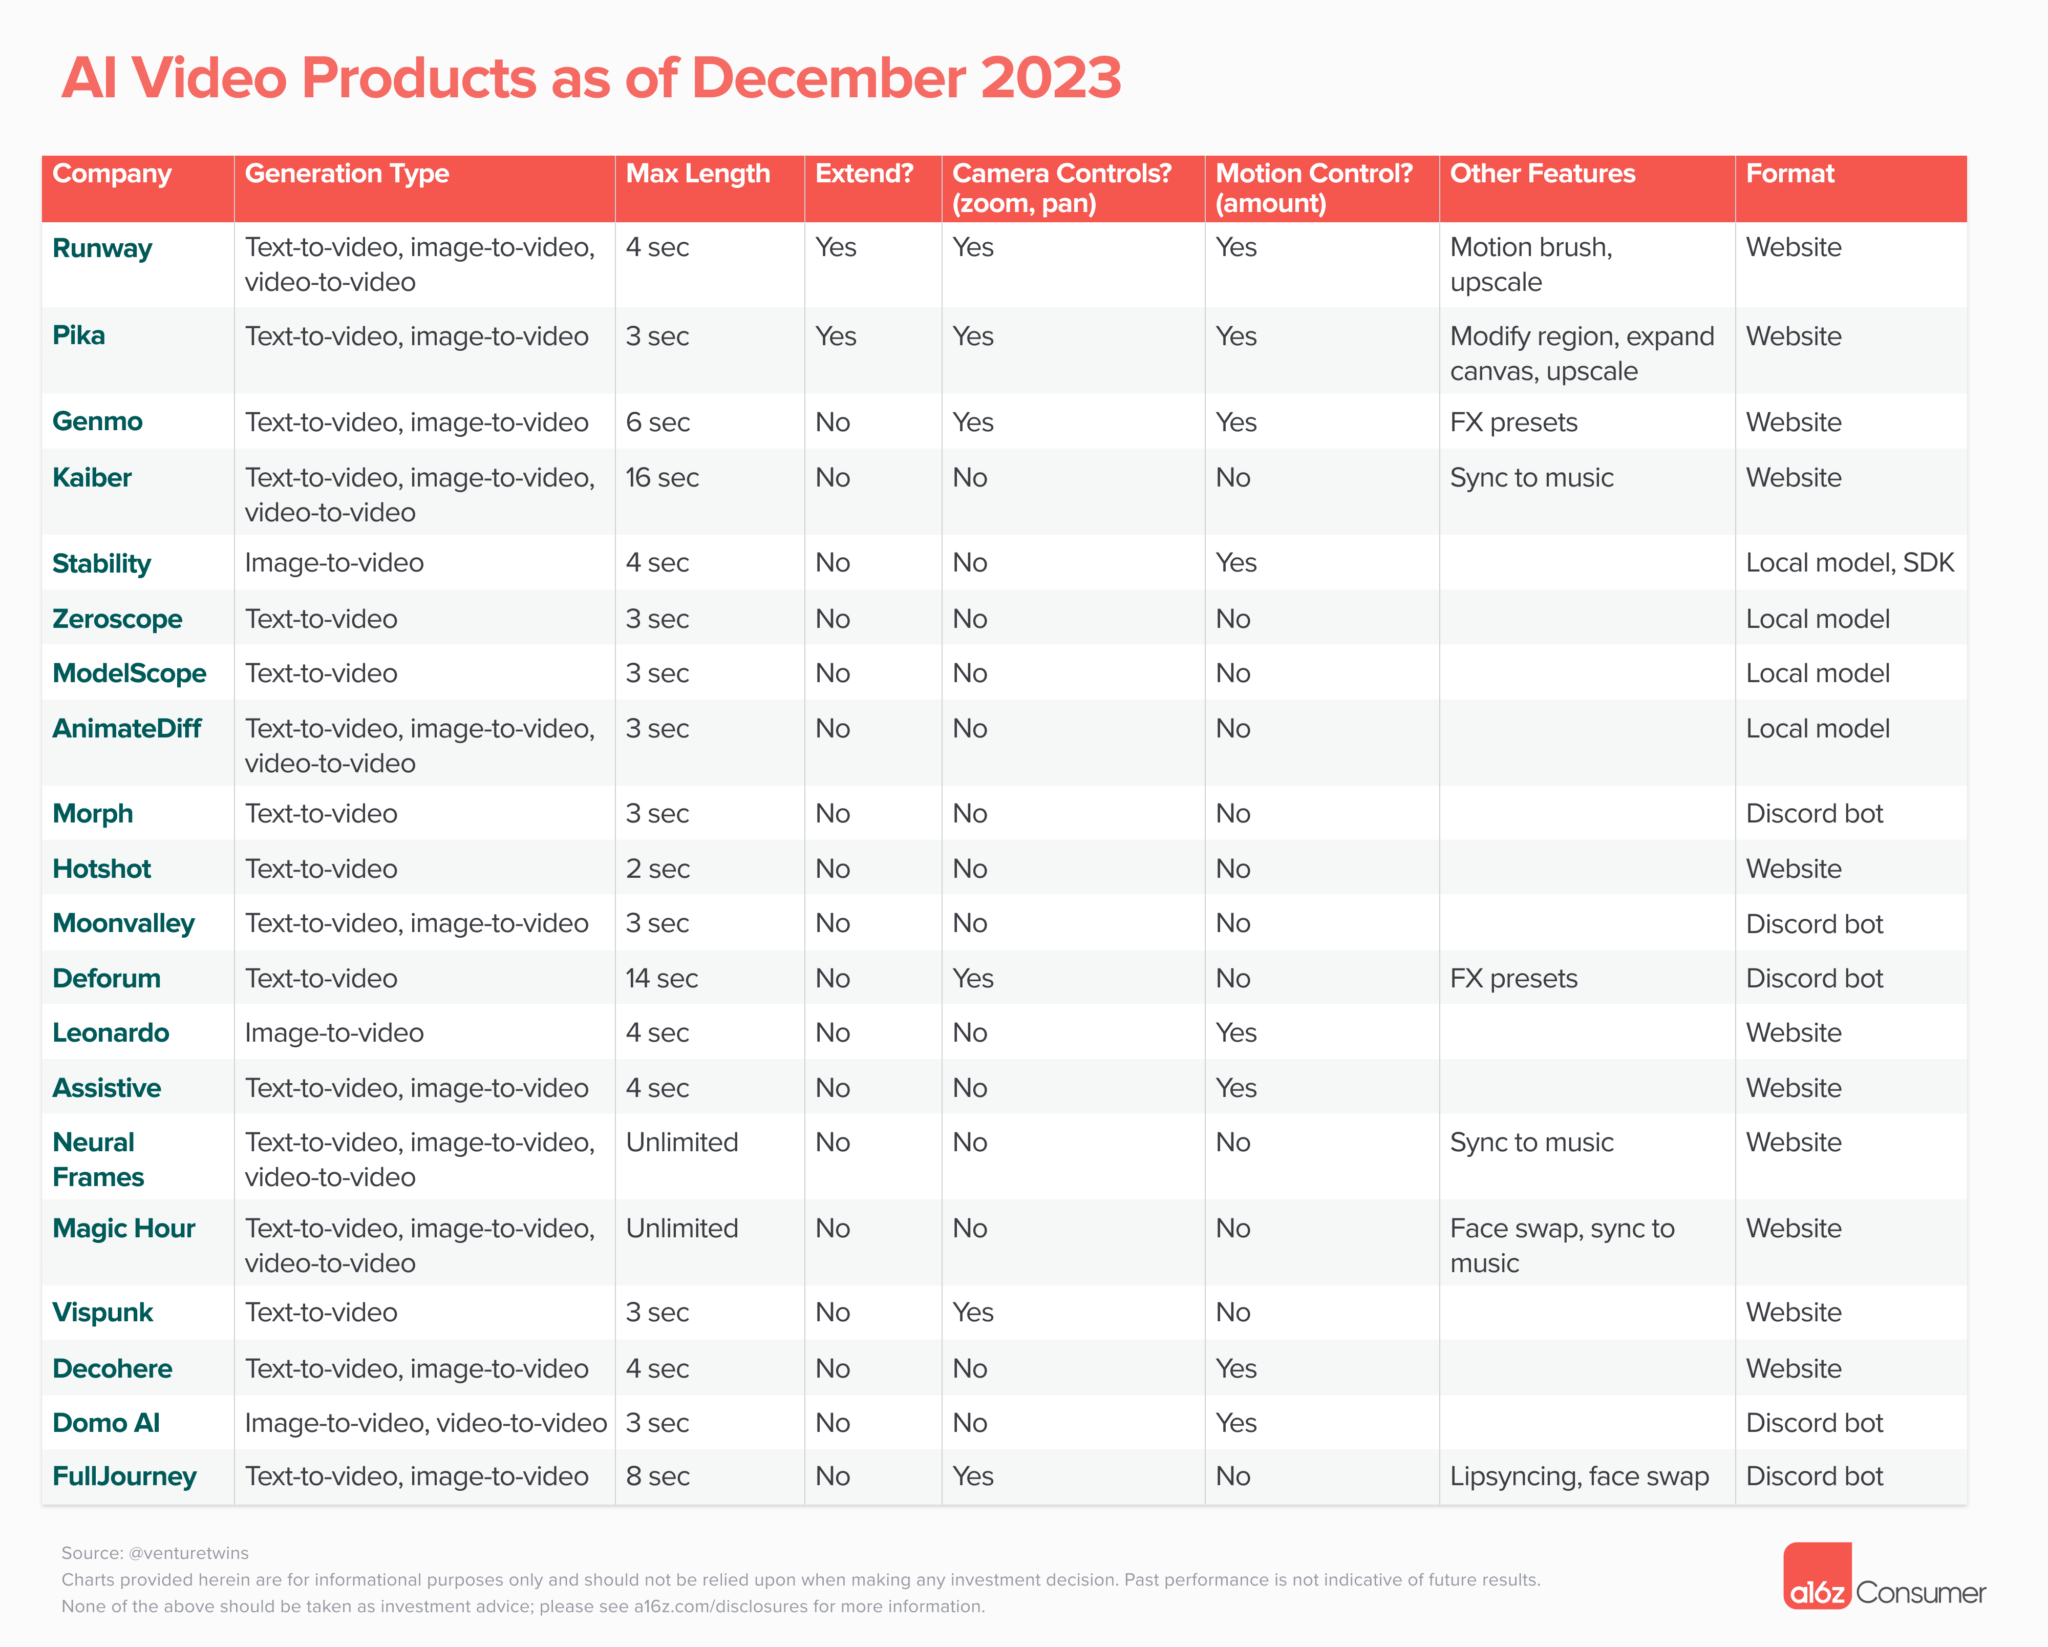
\includegraphics[width=0.8\textwidth]{products.png}
  \caption{Comparative analysis of various AI video product offerings as of December 2023, detailing generation types, maximum length of generated clips, and additional features \cite{a16zAI2023}.}
\end{figure}

The regulatory environment for AI is rapidly evolving, with significant developments in the EU, China, and the US. 
The EU's provisional agreement on the AI Act \cite{eu_ai_act_2023}, China's measures to regulate AI usage \cite{China_AI_Policy_2023}, and the US's executive order on AI governance \cite{WhiteHouse_AI_ExecOrder_2023} reflect a global movement towards establishing legal frameworks to ensure responsible AI development and deployment. 
The outcome of ongoing legal battles, such as the New York Times' lawsuit against OpenAI \cite{Grynbaum_Mac_2023_Times_Sues_OpenAI}, may have far-reaching implications for the future of AI regulation and its impact on innovation and deployment. 
As we look towards the future, the most impactful developments in AI may well be centered around governance, middleware, and data pipelines that make generative AI more trustworthy and accessible. 
With a more refined understanding of AI capabilities, businesses are now focusing on integrating AI tools into existing services to enhance rather than revolutionize established processes. 
The challenge lies in striking a balance between leveraging the unique opportunities presented by AI while managing realistic expectations about its role in reshaping business practices.

\begin{figure}[htbp]
  \centering
  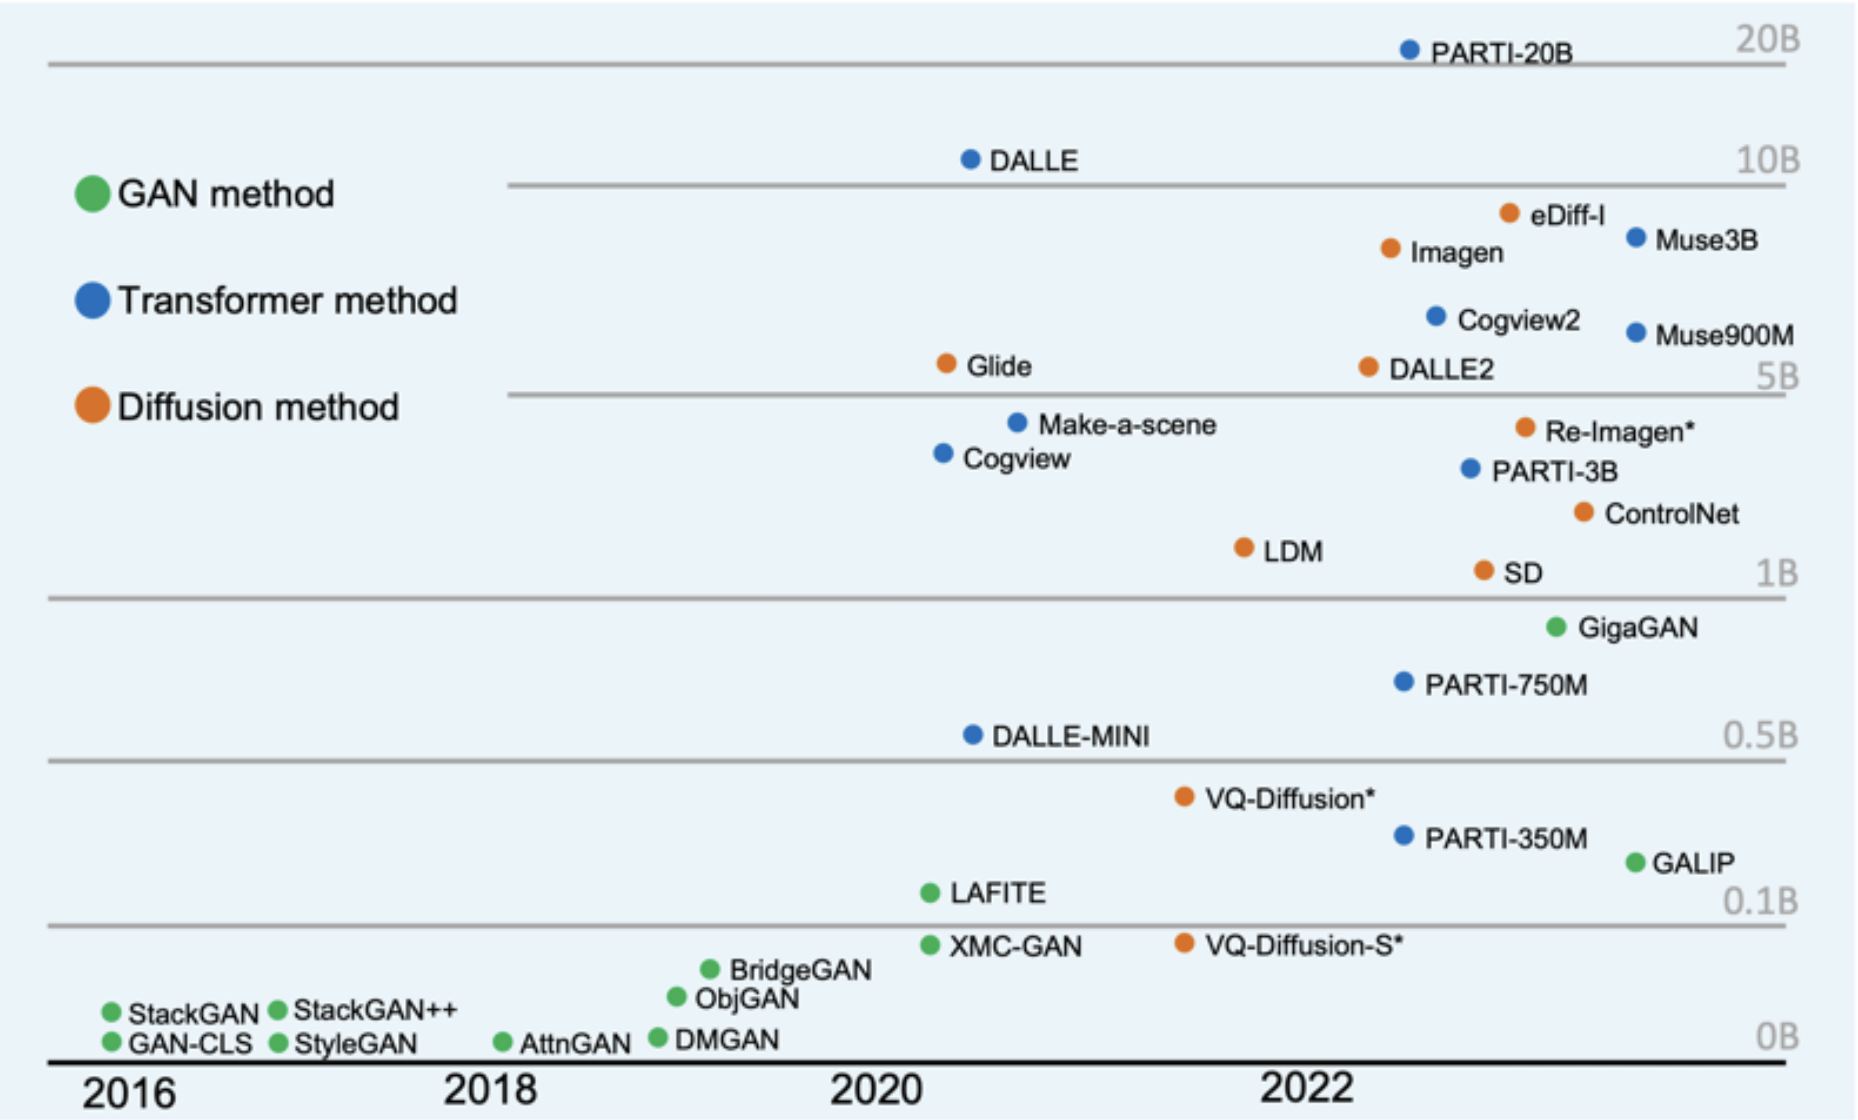
\includegraphics[width=0.8\textwidth]{models.png}
  \caption{Progression of generative modeling techniques from 2016 to 2022, showcasing the evolution and scaling of model parameters in GAN, Transformer, and Diffusion methods, each color-coded by method type \cite{bie2023renaissance}.}
\end{figure}

In the field of image generation, models like Midjourney, DALL-E 3, and Stable Diffusion 3 have been at the forefront. 
Video generation has also seen substantial growth, with platforms such as Runway Gen-2, Pika, and Sora pushing the boundaries of what can be achieved in AI-generated cinematography. 
In the audio domain, AI's capability to replicate and generate human-like speech has made significant strides with models such as ElevenLabs, Speechify, and Whisper. 
These tools have not only democratized voice-over and audio content production but have also raised the bar for what can be expected from synthetic speech in terms of clarity, emotion, and expressiveness. 
The geographical landscape of AI development is also noteworthy, with the United States and China emerging as the primary incubators of AI innovation. 
Leading internet companies in these countries, including tech giants like Google, Meta, Alibaba, and ByteDance, have been instrumental in driving forward the development of AI technologies. 
Their investments have resulted in state-of-the-art models that, while most of them are not open-source.

\section{Case Study: Using AI tools to predict the future of soccer}
In an effort to visualize the potential of AI in the content creating, I create a project to design a one-minute video showcasing what the soccer game might look like in the future through the lens of AI. 
This journey was not just about prediction but also indicate how AI can revolutionize content creation and sports entertainment.
This endeavor was made possible by several AI models, including ChatGPT for scripting, Midjourney for visual images generation, Runway for video editing and synthesis, and Topaz AI for enhancing video quality. 
The project not only demonstrates the capabilities of these AI tools but also offers a glimpse into the future of entertainment. 
The video has been shared on social platforms like YouTube, inviting viewers to engage with and reflect on the evolving intersection of technology and sports.
This case study emphasized that user should treat AI as a colleague during the process, giving the clear and detailed prompts to ensure the result is close to the expectations.
Even though AI tools can inspire the user during the brainstorming, but human still need to have a basic framework before starting the project.
In the end, this project highlights how human creativity combined with AI's efficiency can unlock the opportunities for innovation and engagement in productivity.


\chapter{Methods}

This chapter provides a comprehensive overview of the methodologies and tools utilized in this study to explore the potential of AIGC across various domains including text, image, video, and sound synthesis. 
It outlines the step-by-step process of employing advanced AI models such as GPT-4 for text generation, Midjourney for image creation, Runway Gen-2 for video production, ElevenLabs for voice cloning, and Topaz AI for enhancing visual quality. 
The chapter delves into the technical frameworks underpinning these tools, including Variational Autoencoders (VAE), Generative Adversarial Networks (GAN), and Recurrent Neural Networks (RNN) among others, to illustrate how they contribute to the generation and manipulation of digital content. 
Through a detailed exposition of the workflow, from concept development to content creation and enhancement, this chapter sets the foundation for understanding the capabilities of current AIGC technologies, paving the way for further exploration in the Results and Discussion chapters.

\section{Workflow}

\begin{figure}[H]
\centering
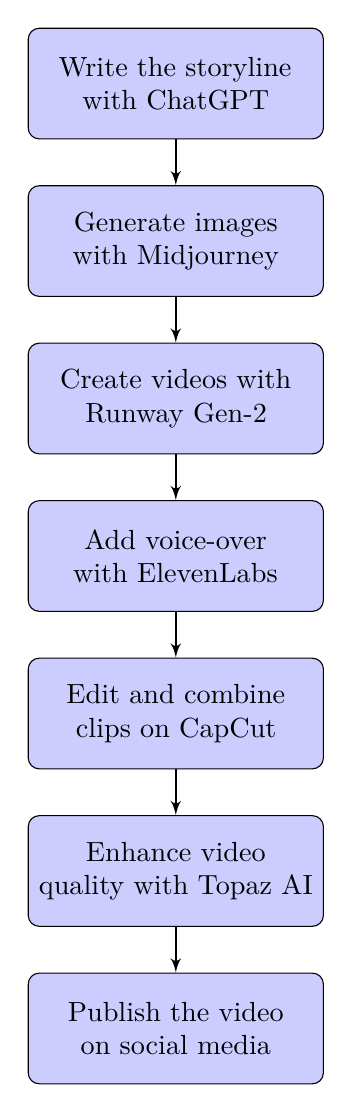
\begin{tikzpicture}[node distance=2cm, auto]
    % Define the style for the nodes
    \tikzstyle{block} = [rectangle, draw, fill=blue!20, text width=10em, text centered, rounded corners, minimum height=4em]
    \tikzstyle{line} = [draw, -latex', thick]
    
    % Place the nodes
    \node [block] (storyline) {Write the storyline with ChatGPT};
    \node [block, below of=storyline] (imagegen) {Generate images with Midjourney};
    \node [block, below of=imagegen] (videogen) {Create videos with Runway Gen-2};
    \node [block, below of=videogen] (voiceover) {Add voice-over with ElevenLabs};
    \node [block, below of=voiceover] (videoedit) {Edit and combine clips on CapCut};
    \node [block, below of=videoedit] (videoquality) {Enhance video quality with Topaz AI};
    \node [block, below of=videoquality] (publish) {Publish the video on social media};
    
    % Connect the nodes with paths
    \path [line] (storyline) -- (imagegen);
    \path [line] (imagegen) -- (videogen);
    \path [line] (videogen) -- (voiceover);
    \path [line] (voiceover) -- (videoedit);
    \path [line] (videoedit) -- (videoquality);
    \path [line] (videoquality) -- (publish);
\end{tikzpicture}
\caption{Workflow of the video-creating project.}
\end{figure}

\begin{figure}[H]
\centering
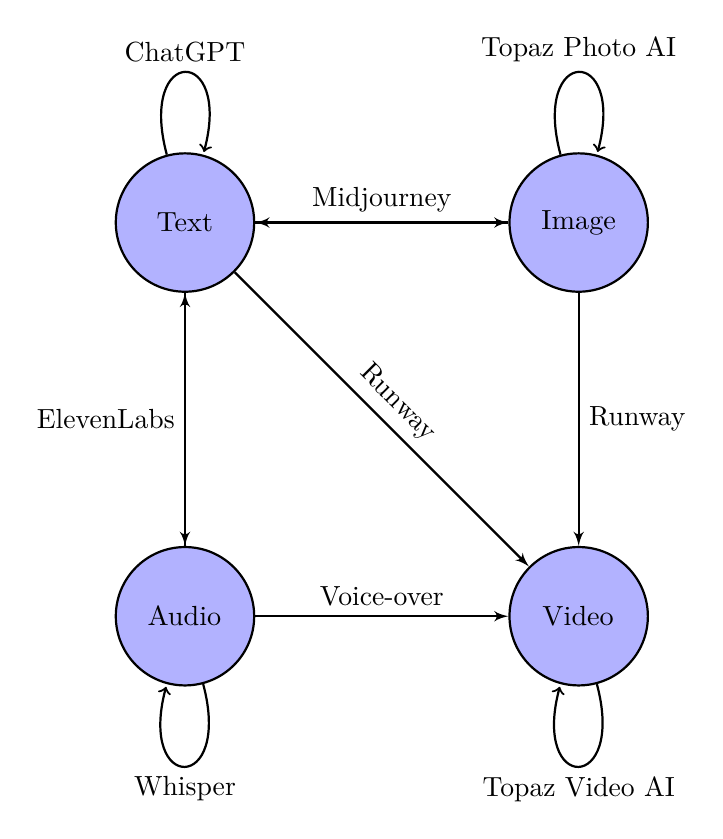
\begin{tikzpicture}[node distance=5cm, auto]
    % Define the style for the nodes
    \tikzstyle{main} = [circle, thick, draw, fill=blue!30, text width=3em, text centered, minimum height=5em]
    \tikzstyle{line} = [draw, -latex', thick]
    
    % Place the nodes
    \node [main] (text) {Text};
    \node [main, right of=text] (image) {Image};
    \node [main, below of=image] (video) {Video};
    \node [main, left of=video] (audio) {Audio};
  
    % Connect the nodes with paths
    \path [line] (text) -- node[above] {Midjourney} (image);
    \path [line] (image) -- (text);
    \path [line] (text) -- (audio);
    \path [line] (text) -- node[sloped, above] {Runway} (video);
    \path [line] (image) -- node[right] {Runway} (video);
    \path [line] (audio) -- node[above] {Voice-over} (video);
    \path [line] (audio) -- node[left] {ElevenLabs} (text);

    \path [line] (text) edge [loop above] node {ChatGPT} (text);
    \path [line] (image) edge [loop above] node {Topaz Photo AI} (image);
    \path [line] (video) edge [loop below] node {Topaz Video AI} (video);
    \path [line] (audio) edge [loop below] node {Whisper} (audio);
  
\end{tikzpicture}
\caption{Relationships in a Multimodal System.}
\end{figure}
Figures 2.1 and 2.2 collectively capture the workflow and the interdependent relationships involved in a multimodal AIGC system. 
Figure 2.1 outlines the sequential workflow, initiating with the drafting of a storyline via ChatGPT, proceeding to image generation with Midjourney, followed by video creation with Runway Gen-2, voice-over addition via ElevenLabs, and concluding with the enhancement of video quality with Topaz AI before the final content is published on social media. 
This flowchart shows the linear progression of tasks, highlighting how each stage builds upon the previous to contribute to the final multimedia product.

\section{AIGC in Text (ChatGPT)}

\subsection{Reinforcement Learning from Human Feedback (RLHF)}

Reinforcement Learning from Human Feedback (RLHF) \cite{christiano2017deep} can align the model's outputs with human preferences. 

The objective of RLHF is to optimize the policy $\pi$ to maximize the expected reward, which is indicative of the alignment between generated outputs and human preferences:

\begin{equation}
\max_{\pi} \mathbb{E}_{\tau \sim \pi} [R(\tau)],
\end{equation}

where $\tau = (s_0, a_0, ..., s_{T-1}, a_{T-1}, s_T)$ represents a trajectory of states and actions, and $R(\tau)$ is the cumulative reward for trajectory $\tau$.

Human feedback is used to train a reward model $R_{\theta}(s,a)$, parameterized by $\theta$, which estimates the reward of taking action $a$ in state $s$:

\begin{equation}
R_{\theta}(s,a) = \text{HumanFeedback}(s, a).
\end{equation}

The policy $\pi_{\phi}$, parameterized by $\phi$, is optimized using the reward model as a surrogate for the true human feedback:

\begin{equation}
\phi^{*} = \arg\max_{\phi} \mathbb{E}_{\tau \sim \pi_{\phi}} [R_{\theta}(s,a)].
\end{equation}

Typically, Proximal Policy Optimization (PPO) or a similar algorithm is employed for policy optimization, ensuring stable and efficient learning:

\begin{equation}
L(\phi) = \hat{\mathbb{E}}_t \left[ \min(r_t(\phi) \hat{A}_t, \text{clip}(r_t(\phi), 1-\epsilon, 1+\epsilon) \hat{A}_t) \right],
\end{equation}

where $r_t(\phi) = \frac{\pi_{\phi}(a_t|s_t)}{\pi_{\phi_{old}}(a_t|s_t)}$ is the probability ratio, $\hat{A}_t$ is the advantage estimate at time $t$, and $\epsilon$ is a hyperparameter that controls clipping to reduce variance.

All the processes above indicate how RLHF is mathematically conceptualized in the context of improving GPT models, focusing on optimizing the model to generate text that aligns with human preferences based on feedback.

\subsection{Transfer Learning}
Given a pretrained model \(M\) with parameters \(\theta\), transfer learning \cite{torrey2010transfer} adjusts \(\theta\) to new parameters \(\theta'\) to better perform on a target task \(T\) with a smaller dataset \(D_{T}\). The objective is to minimize the loss function \(\mathcal{L}_{T}\) on \(D_{T}\), leveraging knowledge from the source task \(S\).

The optimization problem can be formalized as:
\[
\theta' = \arg\min_{\theta} \mathcal{L}_{T}(f_{\theta}(D_{T})),
\]
where \(f_{\theta}\) denotes the model's prediction function parameterized by \(\theta\).

The loss function \(\mathcal{L}_{T}\) often takes the form of cross-entropy in text-based tasks:
\[
\mathcal{L}_{T} = -\frac{1}{N}\sum_{i=1}^{N}\sum_{c=1}^{C} y_{ic}\log(p_{ic}),
\]
where \(N\) is the number of samples in \(D_{T}\), \(C\) is the number of classes, \(y_{ic}\) is a binary indicator of whether class \(c\) is the correct classification for observation \(i\), and \(p_{ic}\) is the predicted probability of observation \(i\) being in class \(c\).

For fine-tuning, we update \(\theta\) with a learning rate \(\alpha\) specific to the target task:
\[
\theta' = \theta - \alpha \nabla_{\theta} \mathcal{L}_{T}(f_{\theta}(D_{T})).
\]

To prevent catastrophic forgetting, a regularization term \(\mathcal{R}(\theta)\) may be added, balancing the new task learning and retention of previously learned knowledge:
\[
\theta' = \arg\min_{\theta} \mathcal{L}_{T}(f_{\theta}(D_{T})) + \lambda \mathcal{R}(\theta),
\]
where \(\lambda\) controls the importance of the regularization term, and \(\mathcal{R}(\theta)\) can be defined as the difference between the new parameters \(\theta'\) and the original pretrained parameters \(\theta\), such as in elastic weight consolidation (EWC):
\[
\mathcal{R}(\theta) = \sum_{i} \frac{1}{2} \Omega_{i} (\theta_{i} - \theta_{i}^{*})^2,
\]
with \(\Omega_{i}\) representing the importance of parameter \(i\) for the tasks learned during pretraining and \(\theta^{*}\) denoting the parameters after pretraining.

Thus, transfer learning efficiently leverages pre-existing knowledge of GPT-4, enabling it to adapt to new tasks with remarkable efficiency and minimal data, bridging the gap between general and specific task performances.

\begin{figure}[htbp]
  \centering
  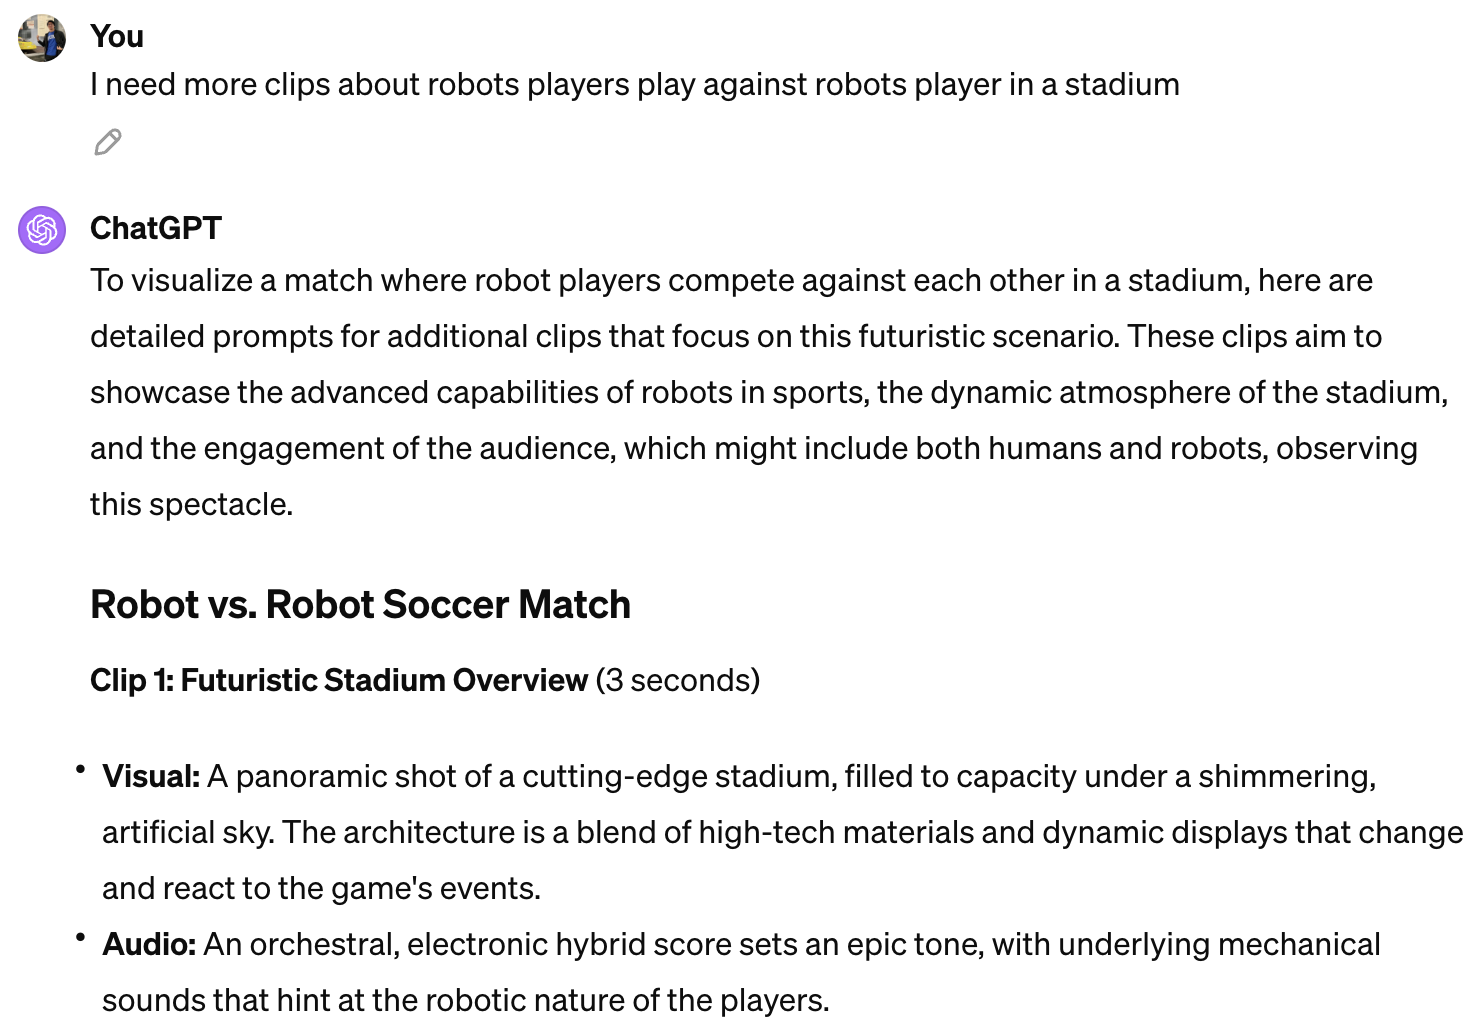
\includegraphics[width=0.8\textwidth]{ChatGPT.png}
  \caption{Using ChatGPT to generate vivid description prompt and prepare for creating the image stills.}
\end{figure}

ChatGPT utilizes Reinforcement Learning from Human Feedback (RLHF) and Transfer Learning to create a highly adaptive and user-aligned conversational model. 
Through RLHF, ChatGPT continuously refines its responses based on broad human feedback, optimizing its conversational results to align more closely with human preferences and expectations. 
This process ensures that the model's outputs are not only relevant but also resonate with users on a more personal level. 
Meanwhile, by employing Transfer Learning, ChatGPT can efficiently adapt to a wide range of conversational contexts and domains with relatively small amounts of task-specific data. 
This dual approach allows ChatGPT to maintain a broad understanding of language and context, gained from its initial training on diverse datasets, while also being able to specialize and improve in specific areas or topics as directed by user interactions and feedback. 
Thus, the integration of RLHF and Transfer Learning enables ChatGPT to offer conversational experiences that are both deeply informed and highly customized, making it a versatile tool for a variety of applications.

\section{AIGC in Image and Video (Midjourney Runway Topaz)}

\subsection{Variational Autoencoders (VAE)}

Variational Autoencoders (VAEs) are a subclass of autoencoders that are foundational for generative models. They are composed of an encoder and a decoder \cite{cho2014properties}. The encoder transforms input data into a latent space, whereas the decoder reconstructs the input data from this space. The latent space is typically modeled as a Gaussian distribution, with the encoder providing the parameters—mean $\mu$ and variance $\sigma^2$—for this distribution.

The encoder part of a VAE is responsible for compressing the input data into a latent representation. For a given data element $x_i$, the encoder produces a mean $\mu_i$ and a variance $\sigma^2_i$ that define a Gaussian distribution in the latent space. The encoding process can be represented by the following equation:
\begin{equation}
\log q_{\phi} \left( z^{(i)} | x^{(i)} \right) = \log \mathcal{N} \left( z^{(i)}; \mu^{(i)}, \sigma^{2(i)} I \right).
\end{equation}

To allow for gradient descent methods to work, VAEs employ a reparameterization trick. This trick involves sampling a noise vector $\epsilon$ from a standard Gaussian distribution and then constructing the latent vector $z_i$ by scaling the noise with the standard deviation and shifting by the mean:
\begin{equation}
z_i = \mu_i + \epsilon \times \sigma_i,
\end{equation}
where $\epsilon \sim \mathcal{N}(0, I)$.

The decoder's goal is to reconstruct the input data from the latent representation. It tries to generate data that is as close as possible to the original input by maximizing the likelihood of the data given the latent space representation.

The training of VAEs involves maximizing the evidence lower bound (ELBO) on the marginal likelihood of the observed data. The ELBO can be represented as follows:
\begin{equation}
\mathcal{L}_b = -D_{KL}(q(z|x)||p(z)) + \frac{1}{L} \sum_{i=1}^{L}(\log P(x|z)).
\end{equation}
Furthermore, the ELBO can be decomposed into two terms: the first being the Kullback-Leibler divergence between the encoder's distribution and the prior distribution of the latent variables, and the second term being the expected log-likelihood of the data given the latent variables. For a latent space with dimensionality $d$, and assuming a standard Gaussian prior, the loss function simplifies to:
\begin{equation}
\mathcal{L}(\theta, x^i) = -\frac{1}{2} \sum_{i=1}^{d} \left( \mu^{2}_{(i)} + \sigma^{2}_{(i)} - \log \sigma^{2}_{(i)} - 1 \right) + \frac{1}{L} \sum_{i=1}^{L} \left( \log P(x^{i} | z) \right).
\end{equation}

Despite their advantages for generative tasks, VAEs have limitations, particularly for image generation. Directly sampling from the Gaussian distribution often results in blurred images. Moreover, there is an information loss when projecting the data to a lower-dimensional latent space, which affects the quality of the reconstruction. However, VAEs find extensive applications in feature extraction and dimensionality reduction, and they can be particularly effective when combined with other generative models such as Generative Adversarial Networks (GANs) or diffusion models.

\begin{figure}[htbp]
  \centering
  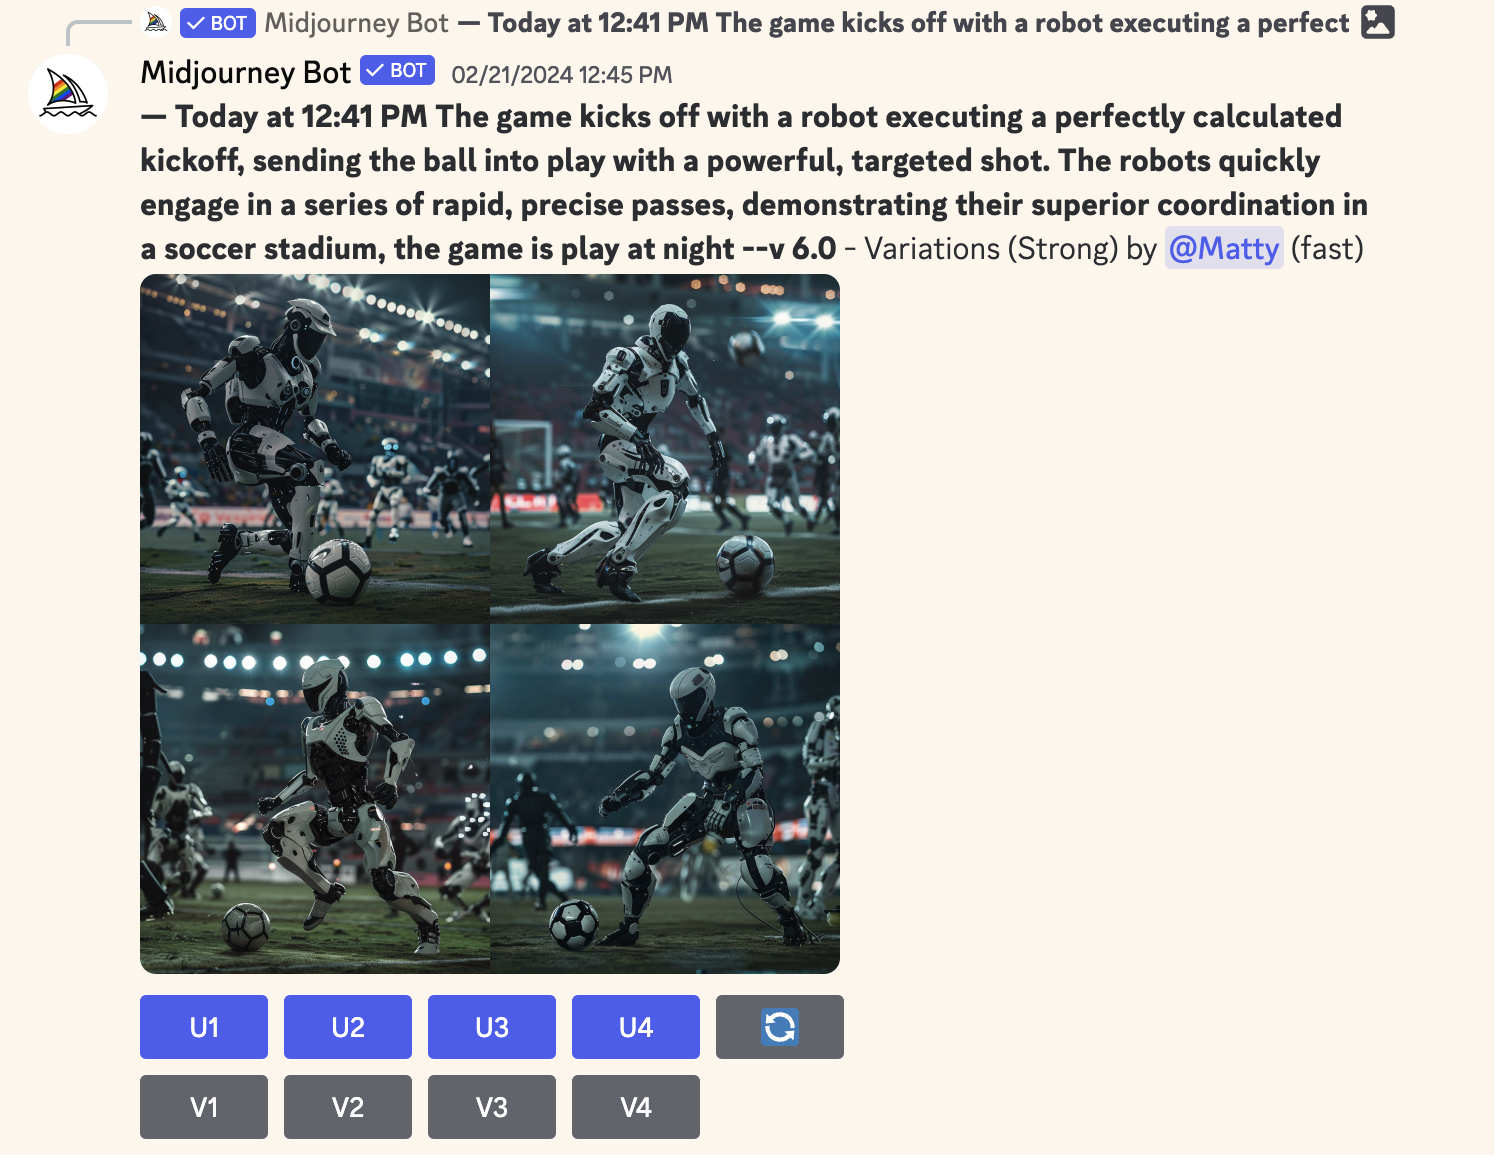
\includegraphics[width=0.8\textwidth]{mj.png}
  \caption{Using ChatGPT's prompts to generate good quality image stills using Midjourney, and then upload them as the key frames to Runway Gen-2 for video clip generation.}
\end{figure}

\subsection{Generative Adversarial Networks (GAN)}

Generative Adversarial Networks (GANs) represent a class of generative models that has significantly impacted the field of synthetic image generation. A GAN is composed of two distinct neural network models: a \textit{generator} ($G$) and a \textit{discriminator} ($D$). The generator attempts to produce data that is indistinguishable from genuine data, while the discriminator evaluates the authenticity of the data, distinguishing between actual and generated samples.

The objective function of a GAN is formulated as a min-max game between $G$ and $D$:
\begin{align}
\min_{G} \max_{D} V(D, G) = \mathbb{E}_{x\sim p_{data}(x)}[\log D(x)] + \mathbb{E}_{z\sim p_{z}(z)}[\log (1 - D(G(z)))],
\end{align}
where $p_{data}$ is the data distribution, $x$ represents real data, $z$ is a noise sample from distribution $p_z$, and $G(z)$ is the generated data.

During training, $D$ is optimized to maximize the probability of correctly classifying a sample as real or fake. Simultaneously, $G$ is optimized to minimize $\log(1 - D(G(z)))$. In practice, this is often achieved by alternating between the following gradient ascent step for $D$:
\begin{align}
\nabla_{\theta_d} \frac{1}{m} \sum_{i=1}^{m} \Big[ \log D(x^{(i)}) + \log (1 - D(G(z^{(i)}))) \Big],
\end{align}
and the gradient descent step for $G$:
\begin{align}
\nabla_{\theta_g} \frac{1}{m} \sum_{i=1}^{m} \log (1 - D(G(z^{(i)}))),
\end{align}
for a minibatch of $m$ samples.

\begin{figure}[htbp]
  \centering
  \includegraphics[width=0.8\textwidth]{GAN.png}
  \caption{The fundamental architecture of a Generative Adversarial Network (GAN) \cite{SemiEngineering2023GAN}.}
\end{figure}

GANs have been utilized to generate high-fidelity images, outperforming other generative models in visual quality. However, they often struggle with mode collapse -- a phenomenon where the generator produces a limited variety of outputs. Despite these challenges, GANs have shown impressive results in tasks beyond image generation, such as image super-resolution \cite{denton2015deep}and object detection \cite{goodfellow2014generative}.

\begin{figure}[htbp]
  \centering
  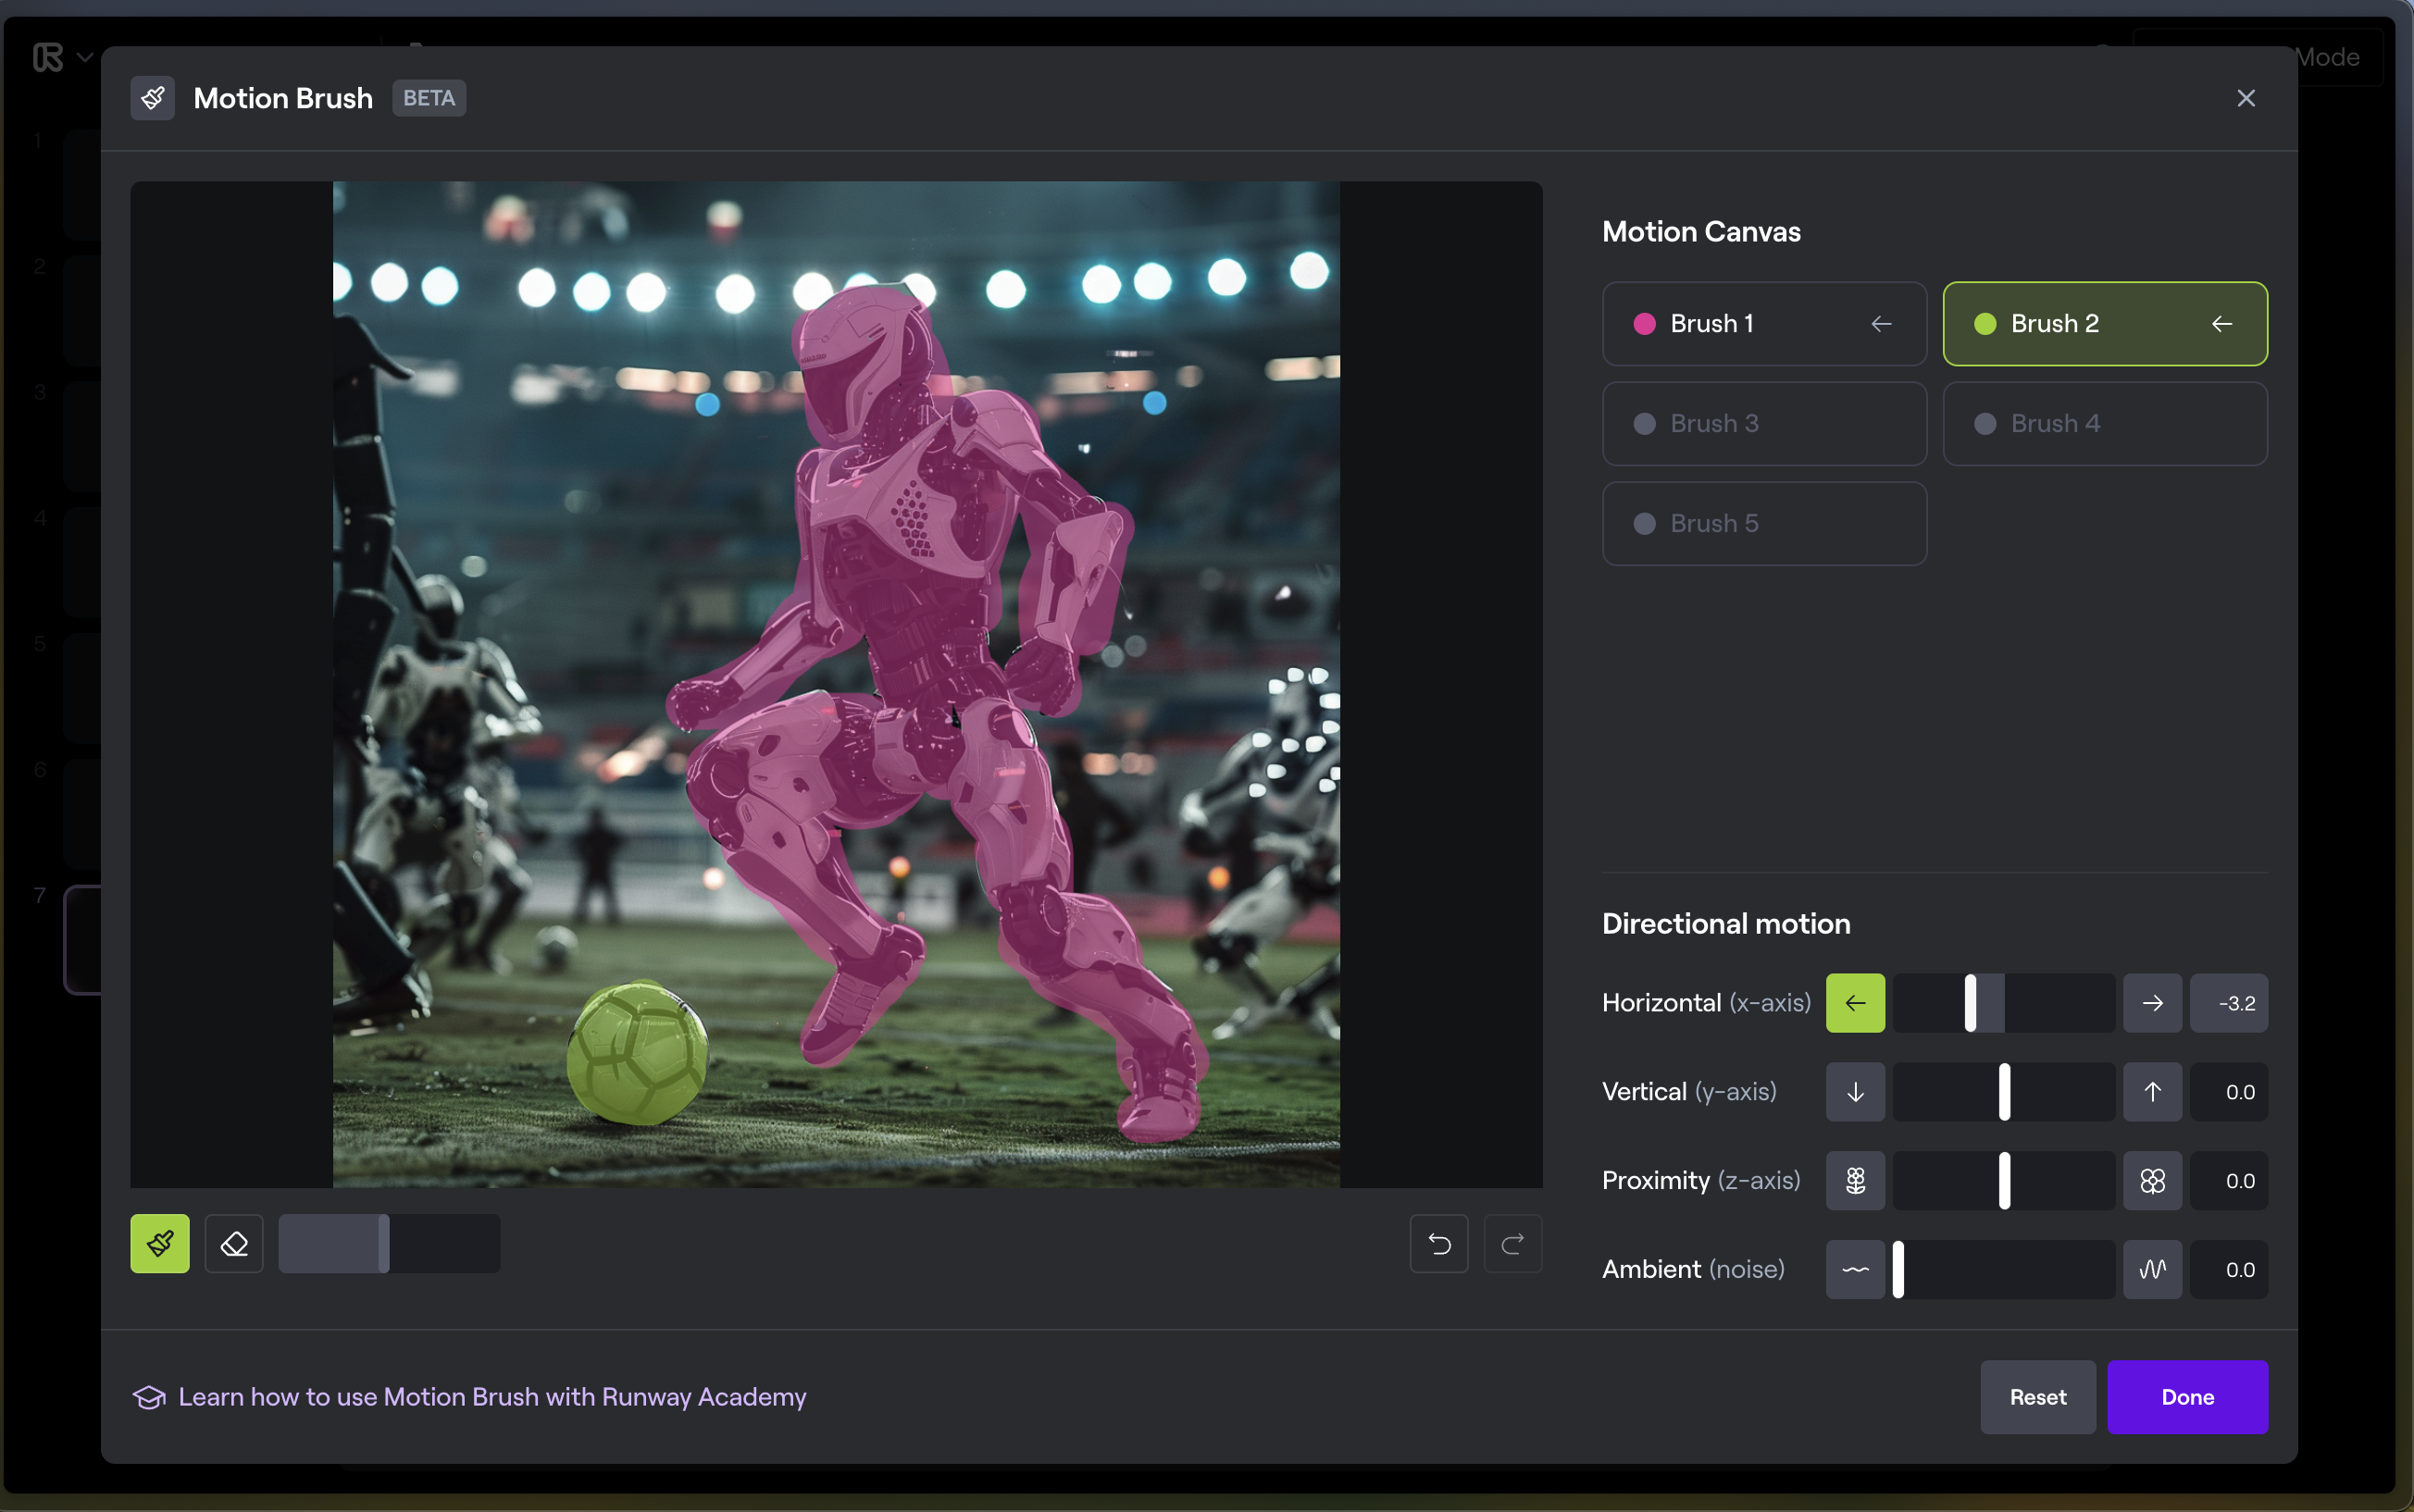
\includegraphics[width=0.8\textwidth]{Runway.png}
  \caption{Using the "Image + Text" mode in Runway Gen-2 to generate the video, with the help of motion brush function to control how the characters move.}
\end{figure}

\subsection{Diffusion Models}

Diffusion models \cite{sohl2015deep, ho2020denoising} are a class of generative models famous for their ability to generate high-quality images through a process that iteratively adds and removes noise. These models are characterized by their use of a Markov chain to gradually convert simple noise distributions into complex data distributions.

A diffusion model typically consists of two main components: the forward process (described in Algorithm 1) and the reverse process (described in Algorithm 2). The forward process models the gradual addition of noise to the data, while the reverse process models the generation of data from noise. Mathematically, the forward process can be described by:
\begin{equation}
q(\mathbf{x}_t | \mathbf{x}_{t-1}) = \mathcal{N}(\mathbf{x}_t; \sqrt{1-\beta_t} \mathbf{x}_{t-1}, \beta_t \mathbf{I}),
\end{equation}
where $\beta_t$ is a variance schedule over discrete timesteps $t = 1, 2, ..., T$. 

\begin{algorithm}
\caption{Diffusion model training \cite{bie2023renaissance}}
\begin{algorithmic}[1]
\STATE for every training iteration do
\STATE \hspace{\algorithmicindent} Sample $t$ from discrete timestep $1, 2, \ldots, T$, or from continuous timestep $t \sim [0, 1]$.
\STATE \hspace{\algorithmicindent} Sample random noise $\epsilon \sim \mathcal{N}(0, 1)$.
\STATE \hspace{\algorithmicindent} Calculate $x_t$ based on DDPM forward or SDE forward.
\STATE \hspace{\algorithmicindent} Update the model with noise prediction $\epsilon(x_t, t)$ or score function $s(x_t, t)$.
\STATE end for
\end{algorithmic}
\label{alg:diffusion_model_training}
\end{algorithm}

The reverse process involves learning a model to reverse this noise addition:
\begin{equation}
p_{\theta}(\mathbf{x}_{t-1} | \mathbf{x}_t) = \mathcal{N}(\mathbf{x}_{t-1}; \mu_{\theta}(\mathbf{x}_t, t), \Sigma_{\theta}(\mathbf{x}_t, t)),
\end{equation}
where $\mu_{\theta}(\mathbf{x}_t, t)$ and $\Sigma_{\theta}(\mathbf{x}_t, t)$ are functions parameterized by a neural network.

\begin{algorithm}
\caption{Diffusion model Inference \cite{bie2023renaissance}}
\begin{algorithmic}[1]
\STATE Sample $x_t$ from normal Gaussian distribution $x_t \sim \mathcal{N}(0, \mathbf{I})$.
\STATE Sample discrete timesteps from $1, 2, \ldots, T$ or continuous timestep from $[0,1]$.
\STATE for $t$ in Reverse(timesteps) do
\STATE \hspace{\algorithmicindent} Calculate the noise distribution $\epsilon(x_t, t)$ or score function $s(x_t, t)$ with the corresponding diffusion model.
\STATE \hspace{\algorithmicindent} Approximate $x_{t-1}$ or $x_{t-\Delta t}$ based on the reverse function.
\STATE end for
\end{algorithmic}
\label{alg:diffusion_model_inference}
\end{algorithm}

The training of diffusion models, as outlined in Algorithm 1, involves adjusting the parameters of the neural network to maximize the likelihood of the data under the reverse process. Similarly, the inference procedure, as outlined in Algorithm 2, utilizes the trained model to generate new data samples by reversing the noise process.

Diffusion models have been applied to a variety of tasks beyond image generation, such as super-resolution and inpainting, demonstrating their versatility and potential in numerous domains of generative modeling.

\begin{figure}[htbp]
  \centering
  \includegraphics[width=0.8\textwidth]{TopazPhoto.png}
  \caption{Using Topaz AI to upscale and improve the video quality, like changing the frame rate from 60 FPS to 120 FPS, removing noise, and sharpen the subject.}
\end{figure}

Midjourney, Runway, and Topaz, while not explicitly disclosing which models they employ, potentially make use of advanced generative models like Variational Autoencoders (VAEs), Generative Adversarial Networks (GANs), and Diffusion Models to offer cutting-edge image and video generation, enhancement, and editing capabilities. 
VAEs could be used to understand and encode the vast complexity of visual data into a manageable latent space, allowing these platforms to efficiently generate or modify content with a deep understanding of visual structures. 
GANs, known for their ability to produce high-quality synthetic images, might be instrumental in enabling these tools to create realistic images and videos that are difficult to distinguish from real ones, enhancing the authenticity and visual appeal of generated content. 
Diffusion Models can be implemented by generating high-fidelity images through iterative refinement and producing coherent visual outputs, particularly useful in tasks like image super-resolution, denoising, and text-to-image (TTI) synthesis. 
The theoretical integration of these models would enable Midjourney, Runway, and Topaz to harness the strengths of each, offering users a versatile tools for creating, enhancing digital media in ways that were previously unimaginable, thus pushing the boundaries of creative and technical possibilities in digital content creation.

\section{AIGC in Sound (ElevenLabs)}

\subsection{Recurrent Neural Networks (RNN)}

Recurrent Neural Networks (RNNs) \cite{srivastava2015unsupervised, chiappa2017recurrent, ha2018world} have shown remarkable capabilities in modeling sequential data, making them particularly suited for applications in sound synthesis. 
Unlike traditional feedforward neural networks, RNNs incorporate a feedback loop, allowing them to maintain a form of memory over input sequences. 
This characteristic is leveraged in sound synthesis to model the temporal dependencies of audio signals, enabling the generation of coherent and dynamic sound sequences.

The fundamental equation governing the operation of a basic RNN unit for sound synthesis can be described as follows:
\begin{equation}
h_t = \sigma(W_{ih} x_t + W_{hh} h_{t-1} + b_h),
\end{equation}
where $h_t$ represents the hidden state at time $t$, $x_t$ is the input vector at time $t$, $W_{ih}$ and $W_{hh}$ are the weights of the input-to-hidden and hidden-to-hidden connections, respectively, $b_h$ is the bias, and $\sigma$ denotes the activation function, often a non-linear function such as the tanh or ReLU.

The output of the RNN, which corresponds to the synthesized sound at each timestep, is computed as:
\begin{equation}
y_t = W_{ho} h_t + b_o,
\end{equation}
where $y_t$ is the output vector at time $t$, $W_{ho}$ represents the weights of the hidden-to-output connections, and $b_o$ is the output bias. \\
To enhance the model's capacity to handle long-term dependencies, which are prevalent in complex sound sequences, Long Short-Term Memory (LSTM) \cite{yu2019review} units or Gated Recurrent Units (GRUs) \cite{dey2017gate} can be incorporated. 
These advanced variants of RNNs introduce mechanisms such as forget gates (in LSTMs) and update gates (in GRUs) that allow the network to selectively remember or forget information. 
This capability significantly improves the network's ability to model sequences with long-range temporal dependencies, making it highly effective for tasks like sound synthesis where the coherence over time is crucial.

\begin{figure}[htbp]
  \centering
  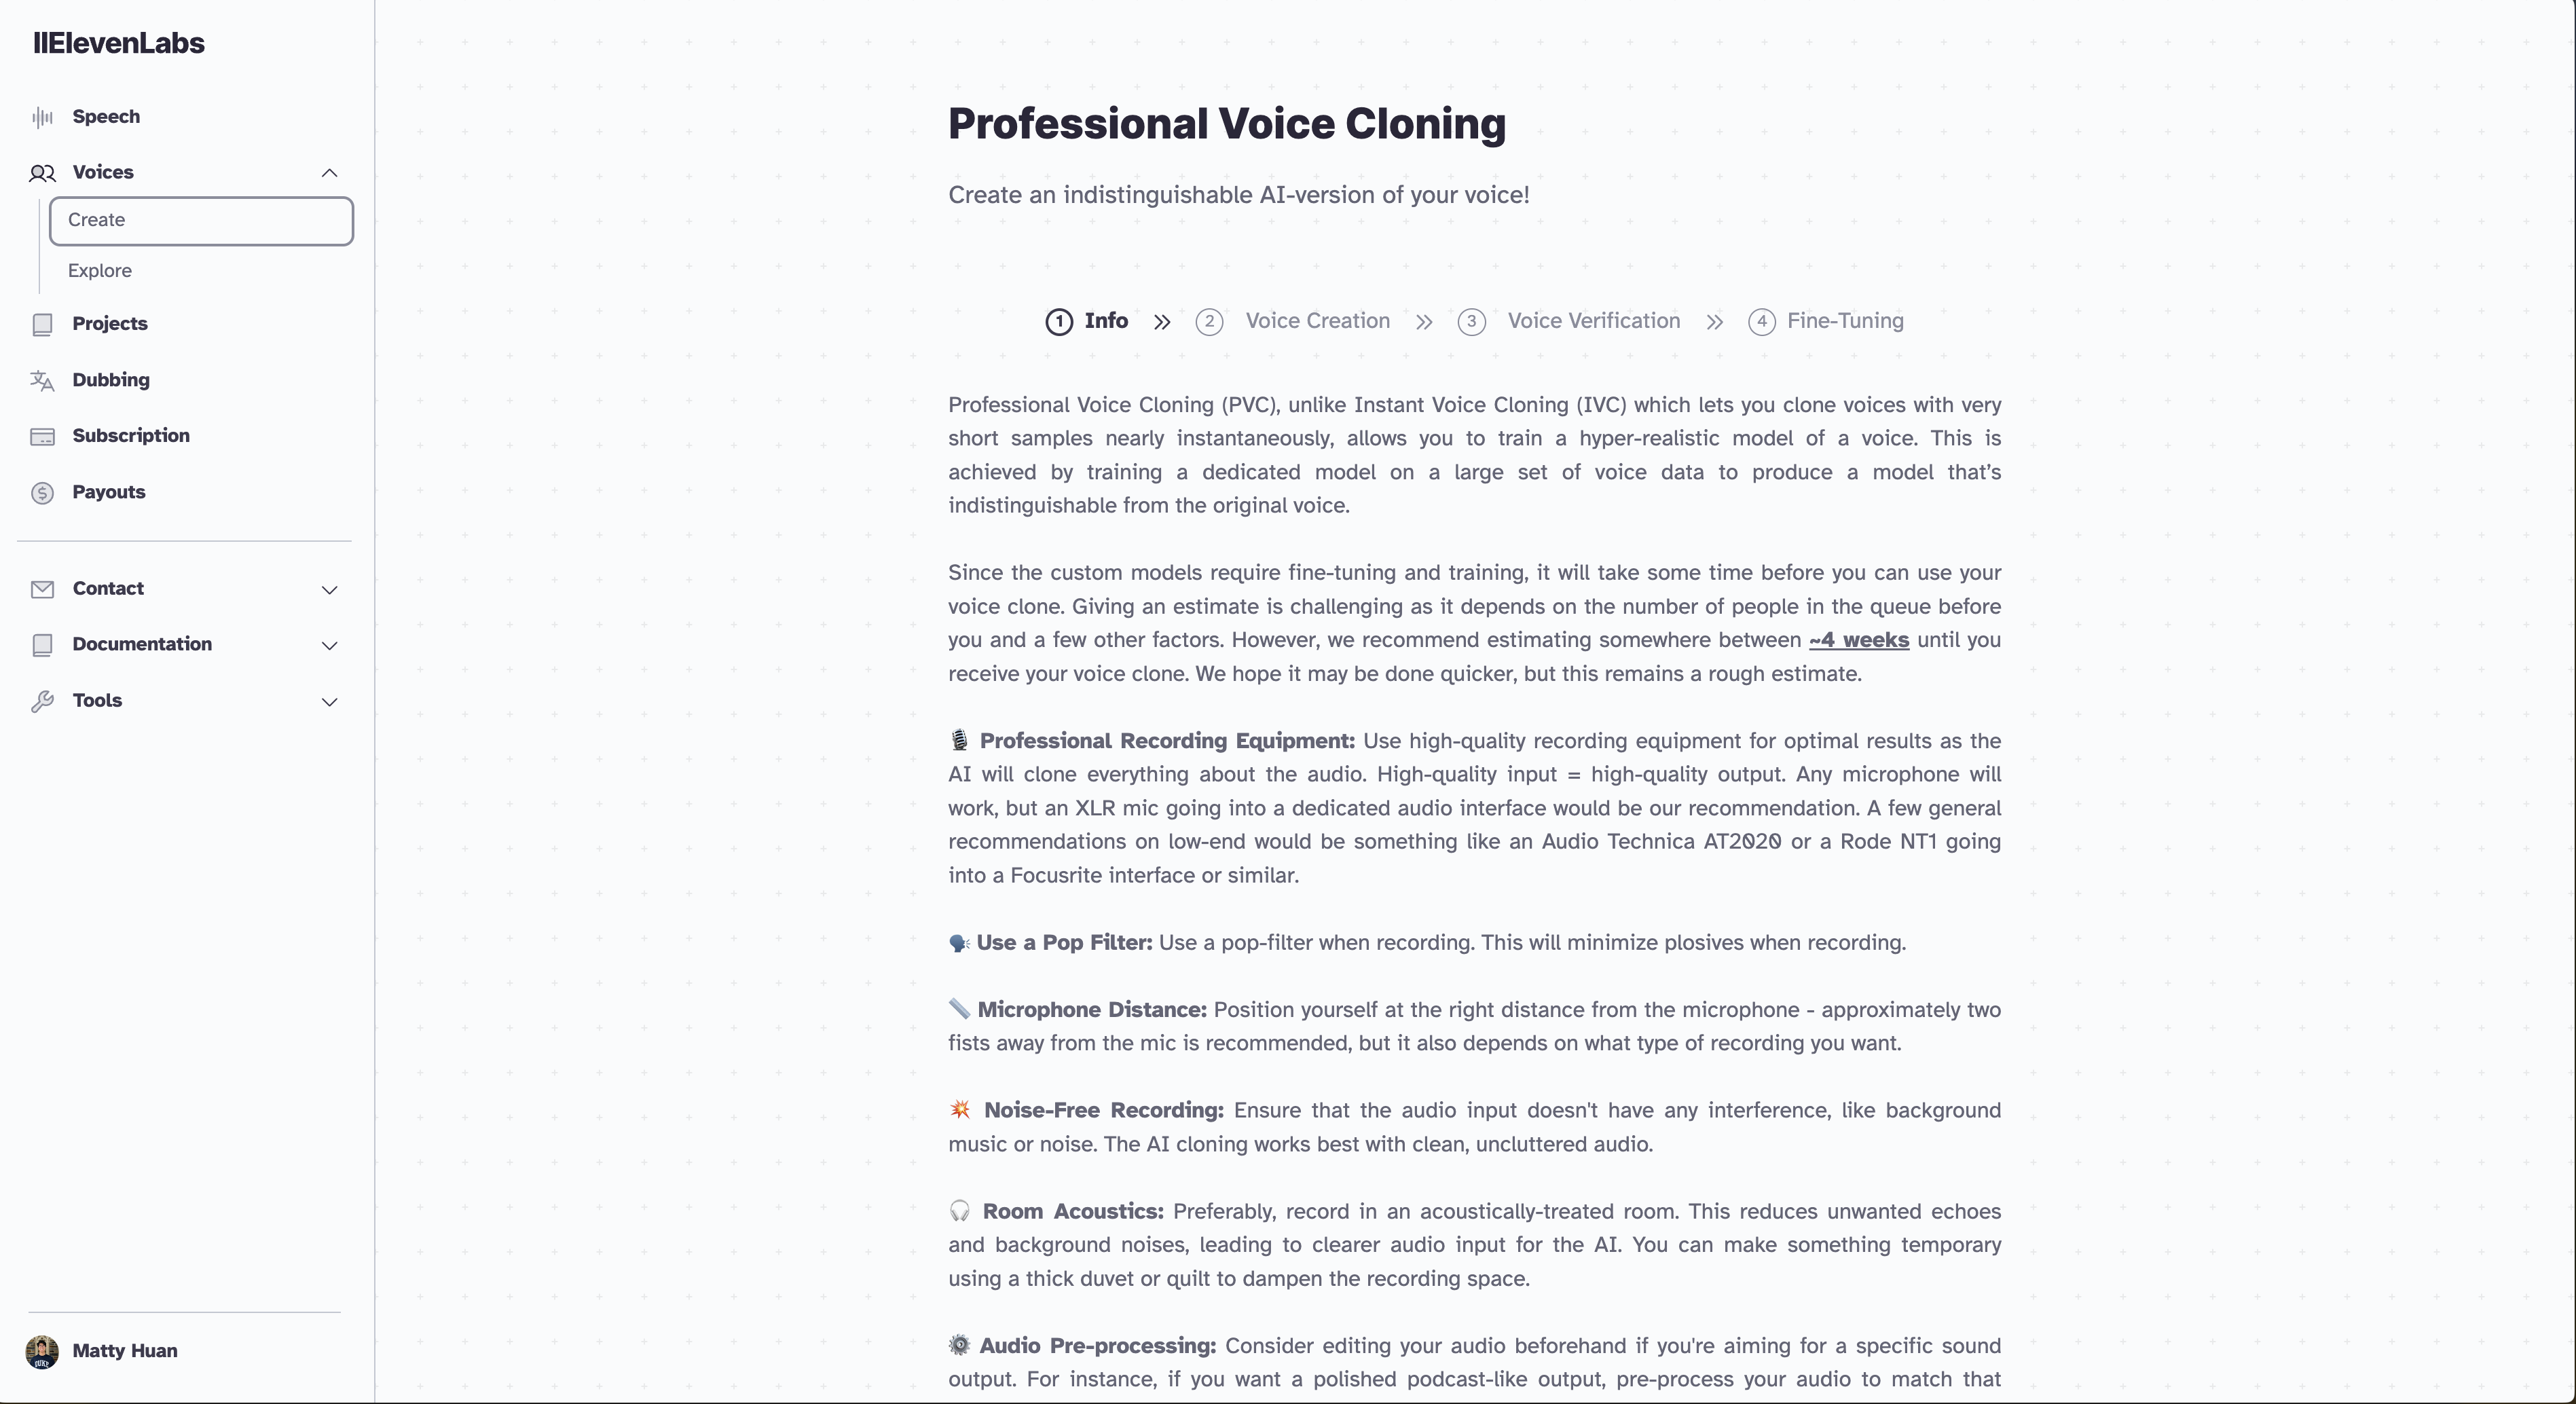
\includegraphics[width=0.6\textwidth]{Voice Cloning.png}
  \caption{Using Professinal Voice Cloning from ElevenLabs to apply text to speech and add the voice over to the video.}
\end{figure}

\begin{figure}[htbp]
  \centering
  \includegraphics[width=0.6\textwidth]{Voice Cloning2.png}
  \caption{Using Professinal Voice Cloning from ElevenLabs to apply text to speech and add the voice over to the video.}
\end{figure}

\subsection{Long Short-Term Memory (LSTM)}

Long Short-Term Memory (LSTM) units are a specific type of Recurrent Neural Network (RNN) architecture designed to overcome the limitations of traditional RNNs, particularly in handling long-term dependencies. LSTMs are adept at modeling the temporal relationships inherent in complex sound sequences, making them highly effective for sound synthesis tasks. The LSTM's architecture includes several key components—forget gate, input gate, cell state, and output gate—that work together to regulate the flow of information through the unit. These components allow the LSTM to retain or discard information over long sequences, enabling the generation of coherent and dynamic audio content. The following equations provide a detailed mathematical representation of the LSTM's operation:

\begin{figure}[htbp]
  \centering
  \includegraphics[width=0.6\textwidth]{LSTM.png}
  \caption{The fundamental structure of LSTM model \cite{wikidocs2023deeplearning}.}
\end{figure}

Forget Gate:
\begin{equation}
f_t = \sigma(W_{f} \cdot [h_{t-1}, x_t] + b_f).
\end{equation}
It decides which information from the cell state is to be discarded. $f_t$ represents the forget gate's activation at time $t$. $\sigma$ is the sigmoid function, $W_{f}$ is the weight matrix for the forget gate, $h_{t-1}$ is the previous hidden state, $x_t$ is the current input, and $b_f$ is the bias.

Input Gate:
\begin{equation}
i_t = \sigma(W_{i} \cdot [h_{t-1}, x_t] + b_i),
\end{equation}
\begin{equation}
\tilde{C}_t = \tanh(W_{C} \cdot [h_{t-1}, x_t] + b_C).
\end{equation}
It controls the extent to which new information is stored in the cell state. $i_t$ is the input gate's activation, and $\tilde{C}_t$ is the candidate value for addition to the cell state. $W_{i}$ and $W_{C}$ are the weight matrices, and $b_i$ and $b_C$ are biases.

Cell State Update:
\begin{equation}
C_t = f_t \ast C_{t-1} + i_t \ast \tilde{C}_t.
\end{equation}
It is updated by removing information deemed unnecessary by the forget gate and adding new candidate values scaled by the input gate's activation.

Output Gate:
\begin{equation}
o_t = \sigma(W_{o} \cdot [h_{t-1}, x_t] + b_o),
\end{equation}
\begin{equation}
h_t = o_t \ast \tanh(C_t).
\end{equation}
It determines the next hidden state $h_t$, which contains information about the current input and the previous state, to be passed to the network. The output gate's activation $o_t$ scales the tanh of the updated cell state, deciding the part of the cell state to output.

In sound synthesis applications, LSTM models are trained on large datasets of audio samples, allowing them to learn and generate new sound sequences that closely mimic the characteristics of the training data. The ability to model long-term dependencies makes LSTMs particularly suited for generating complex and temporally coherent sound sequences, such as musical compositions or natural speech patterns. By optimizing the LSTM parameters (weights and biases) through backpropagation, the model can be fine-tuned to produce high-quality audio outputs that capture the nuances of human-generated sounds.

\subsection{Autoregressive Transformers}

Autoregressive Transformers \cite{yan2021videogpt, wu2022nuwa} have improved sound synthesis by leveraging self-attention mechanisms to model complex sequential data. Unlike RNNs, Transformers process sequences in parallel, allowing for more efficient training and better handling of long-term dependencies. 
In sound synthesis, autoregressive Transformers predict subsequent audio samples based on a sequence of past samples, capturing the temporal dynamics of sound.
The core concept of the Transformer architecture in sound synthesis can be described by the following equations about the self-attention mechanism and the generation process:

Input Embedding and Positional Encoding:
\begin{equation}
X' = X + PE,
\end{equation}
where $X$ is the input sequence of sound samples or features, and $PE$ is the positional encoding added to $X$ to retain positional information.

Self-Attention Mechanism:
\begin{equation}
\text{Attention}(Q, K, V) = \text{softmax}\left(\frac{QK^T}{\sqrt{d_k}}\right)V,
\end{equation}
where $Q$, $K$, and $V$ represent the queries, keys, and values matrices obtained from $X'$, respectively, and $d_k$ is the dimension of the key vectors. This equation calculates the attention weights and applies them to the values to produce an output that highlights important features of the input sequence.

Multi-Head Attention:
\begin{equation}
\text{MultiHead}(Q, K, V) = \text{Concat}(\text{head}_1, \ldots, \text{head}_h)W^O,
\end{equation}
\begin{equation}
\text{head}_i = \text{Attention}(QW^Q_i, KW^K_i, VW^V_i).
\end{equation}
Multi-head attention allows the model to focus on different positions, capturing various aspects of the sound sequence. $W^Q_i$, $W^K_i$, $W^V_i$, and $W^O$ are parameter matrices for each head $i$ and the output projection, respectively.

Position-wise Feed-Forward Networks:
\begin{equation}
\text{FFN}(x) = \max(0, xW_1 + b_1)W_2 + b_2.
\end{equation}
Each layer in the Transformer includes a feed-forward network applied to each position separately and identically. This consists of two linear transformations with a ReLU activation in between.

Output Generation:
\begin{equation}
P(y_t | y_{<t}) = \text{softmax}(y_{t-1}W + b).
\end{equation}
The output at each timestep $t$, $y_t$, is predicted based on the previous outputs $y_{<t}$, where $W$ and $b$ are the weights and bias in the final linear layer that projects the decoder output to the space of possible audio samples. $P(y_t | y_{<t})$ represents the probability distribution over possible next samples given the previous samples.

Training and Fine-tuning:

During pre-training, the model learns to predict the next word in a sentence given the previous words, using a masked language modeling objective:

\begin{equation}
L_{\text{MLM}} = -\sum_{i \in M} \log P(w_i | w_{\setminus i}; \Theta),
\end{equation}

where $M$ denotes the set of masked positions, $w_i$ is the word at position $i$, $w_{\setminus i}$ represents the sequence without the word at position $i$, and $\Theta$ are the model parameters.

Fine-tuning adjusts the pre-trained model to specific tasks or datasets. This phase enhances the model's performance on tasks such as conversational responses, sentiment analysis, and text summarization:

\begin{equation}
L_{\text{task}} = \sum_{(x, y) \in D_{\text{task}}} \log P(y | x; \Theta'),
\end{equation}

where $D_{\text{task}}$ is the task-specific dataset, $(x, y)$ are the input-output pairs, and $\Theta'$ are the fine-tuned model parameters.

By training on sequences of audio samples, autoregressive Transformers learn to generate new sound sequences sample by sample, offering a powerful framework for high-quality sound synthesis, including music composition and speech generation, with the ability to capture the long-range dependencies characteristic of audio signals.

\subsection{Voice Cloning \& Text-to-Speech (TTS)}

The applications of AI-driven voice synthesis, particularly through voice cloning and text-to-speech (TTS) technologies like ElevenLabs \cite{elevenlabs} and Whisper \cite{OpenAIWhisper}, has apparently closed the gap between synthetic and human speech. 
These systems utilize deep learning frameworks to analyze and replicate the nuances of human speech, including tonality and emotion. 
Voice cloning involves creating a digital replica of a target voice from a limited set of audio samples. 
The process can be described by the following stages:

Feature Extraction:
\begin{equation}
F = \text{MFCC}(S),
\end{equation}
where $F$ represents the feature matrix extracted from the input speech signal $S$, and MFCC denotes the Mel-Frequency Cepstral Coefficients, a common feature used in voice synthesis to capture the timbral aspects of the speech.

Acoustic Modeling:
\begin{equation}
H = \text{Encoder}(F; \theta_e),
\end{equation}
\begin{equation}
\tilde{F} = \text{Decoder}(H; \theta_d).
\end{equation}
where $H$ is the encoded representation of the speech features, $\theta_e$ and $\theta_d$ are the parameters of the encoder and decoder networks, respectively, and $\tilde{F}$ is the reconstructed feature matrix. The encoder-decoder framework is often implemented using deep neural networks, where the encoder learns a compressed representation of the speech features, and the decoder reconstructs the features, potentially in the target voice's style.

Voice Conversion:
\begin{equation}
V_t = \text{Conversion}(H_t; \theta_c),
\end{equation}
where $V_t$ represents the target voice features, $H_t$ is the encoded representation of the target speech, and $\theta_c$ are the parameters of the conversion model that transforms the source voice into the target voice.

Waveform Generation:
\begin{equation}
\hat{S} = \text{WaveNet}(V_t; \theta_w),
\end{equation}
where $\hat{S}$ is the synthesized speech waveform, and $\theta_w$ are the parameters of a WaveNet \cite{oord2016wavenet} model trained to convert the feature representation $V_t$ back into the time-domain signal. WaveNet, a deep generative model of raw audio waveforms, is particularly effective in generating high-fidelity speech with natural intonations and expressions.

\begin{figure}[htbp]
  \centering
  \includegraphics[width=0.75\textwidth]{whisper.png}
  \caption{Autoregressive transformer model architecture used for audio processing tasks like transcription and voice synthesis. The model utilizes a stack of encoder and decoder blocks \cite{OpenAIWhisper}.}
\end{figure}

The process of voice cloning and modification enables the generation of synthetic speech that closely resembles a target human voice. 
By capturing the subtle nuances of speech, AI-driven voice synthesis technologies have opened new avenues for creating engaging and emotionally resonant digital communication experiences. 



\subsection{Audio Modification}

There are several methods to tackle audio modification challenges such as noise reduction, sound separation, and audio restoration \cite{godsill2002digital}. 
The processes are shown below:

Noise reduction aims to eliminate unwanted background noise from audio recordings, enhancing the clarity of the sound. This can be mathematically represented by:
\begin{equation}
S_{clean} = S_{noisy} - N,
\end{equation}
where $S_{clean}$ is the clean audio signal, $S_{noisy}$ is the original noisy signal, and $N$ represents the noise component. Advanced AI models, such as Deep Neural Networks (DNNs), are trained to estimate $N$ accurately from $S_{noisy}$, allowing for effective noise removal.

Sound separation involves isolating individual sound sources from a mixed audio signal. This can be expressed as:
\begin{equation}
S_i = F(S_{mix}; \theta_i),
\end{equation}
where $S_i$ is the isolated sound of source $i$, $S_{mix}$ is the mixed audio signal, and $F$ is a function modeled by the AI system with parameters $\theta_i$ tailored to extract the $i^{th}$ sound source.

Audio restoration focuses on recovering the original quality of degraded audio recordings. The process can be conceptualized as:
\begin{equation}
S_{restored} = R(S_{degraded}; \theta_r),
\end{equation}
where $S_{restored}$ is the restored audio signal, $S_{degraded}$ is the degraded audio signal, and $R$ represents the restoration function implemented by the AI with parameters $\theta_r$. This function aims to reconstruct lost or corrupted signal components, effectively restoring the audio to its original state.

The final step often involves enhancing the waveform directly to improve the overall audio quality, which can be mathematically described by:
\begin{equation}
\hat{S} = G(S_{processed}; \theta_g),
\end{equation}
where $\hat{S}$ is the enhanced audio waveform, $S_{processed}$ is the audio signal after noise reduction, sound separation, and restoration, and $G$ is the enhancement function driven by AI with parameters $\theta_g$. Models like WaveNet are examples of generative networks that can be used for this purpose, fine-tuning the audio quality by adjusting the waveform directly.

These core processes involved in audio modification, demonstrating how AI algorithms can significantly improve the clarity, fidelity, and overall quality of sound recordings. 

\begin{figure}[htbp]
  \centering
  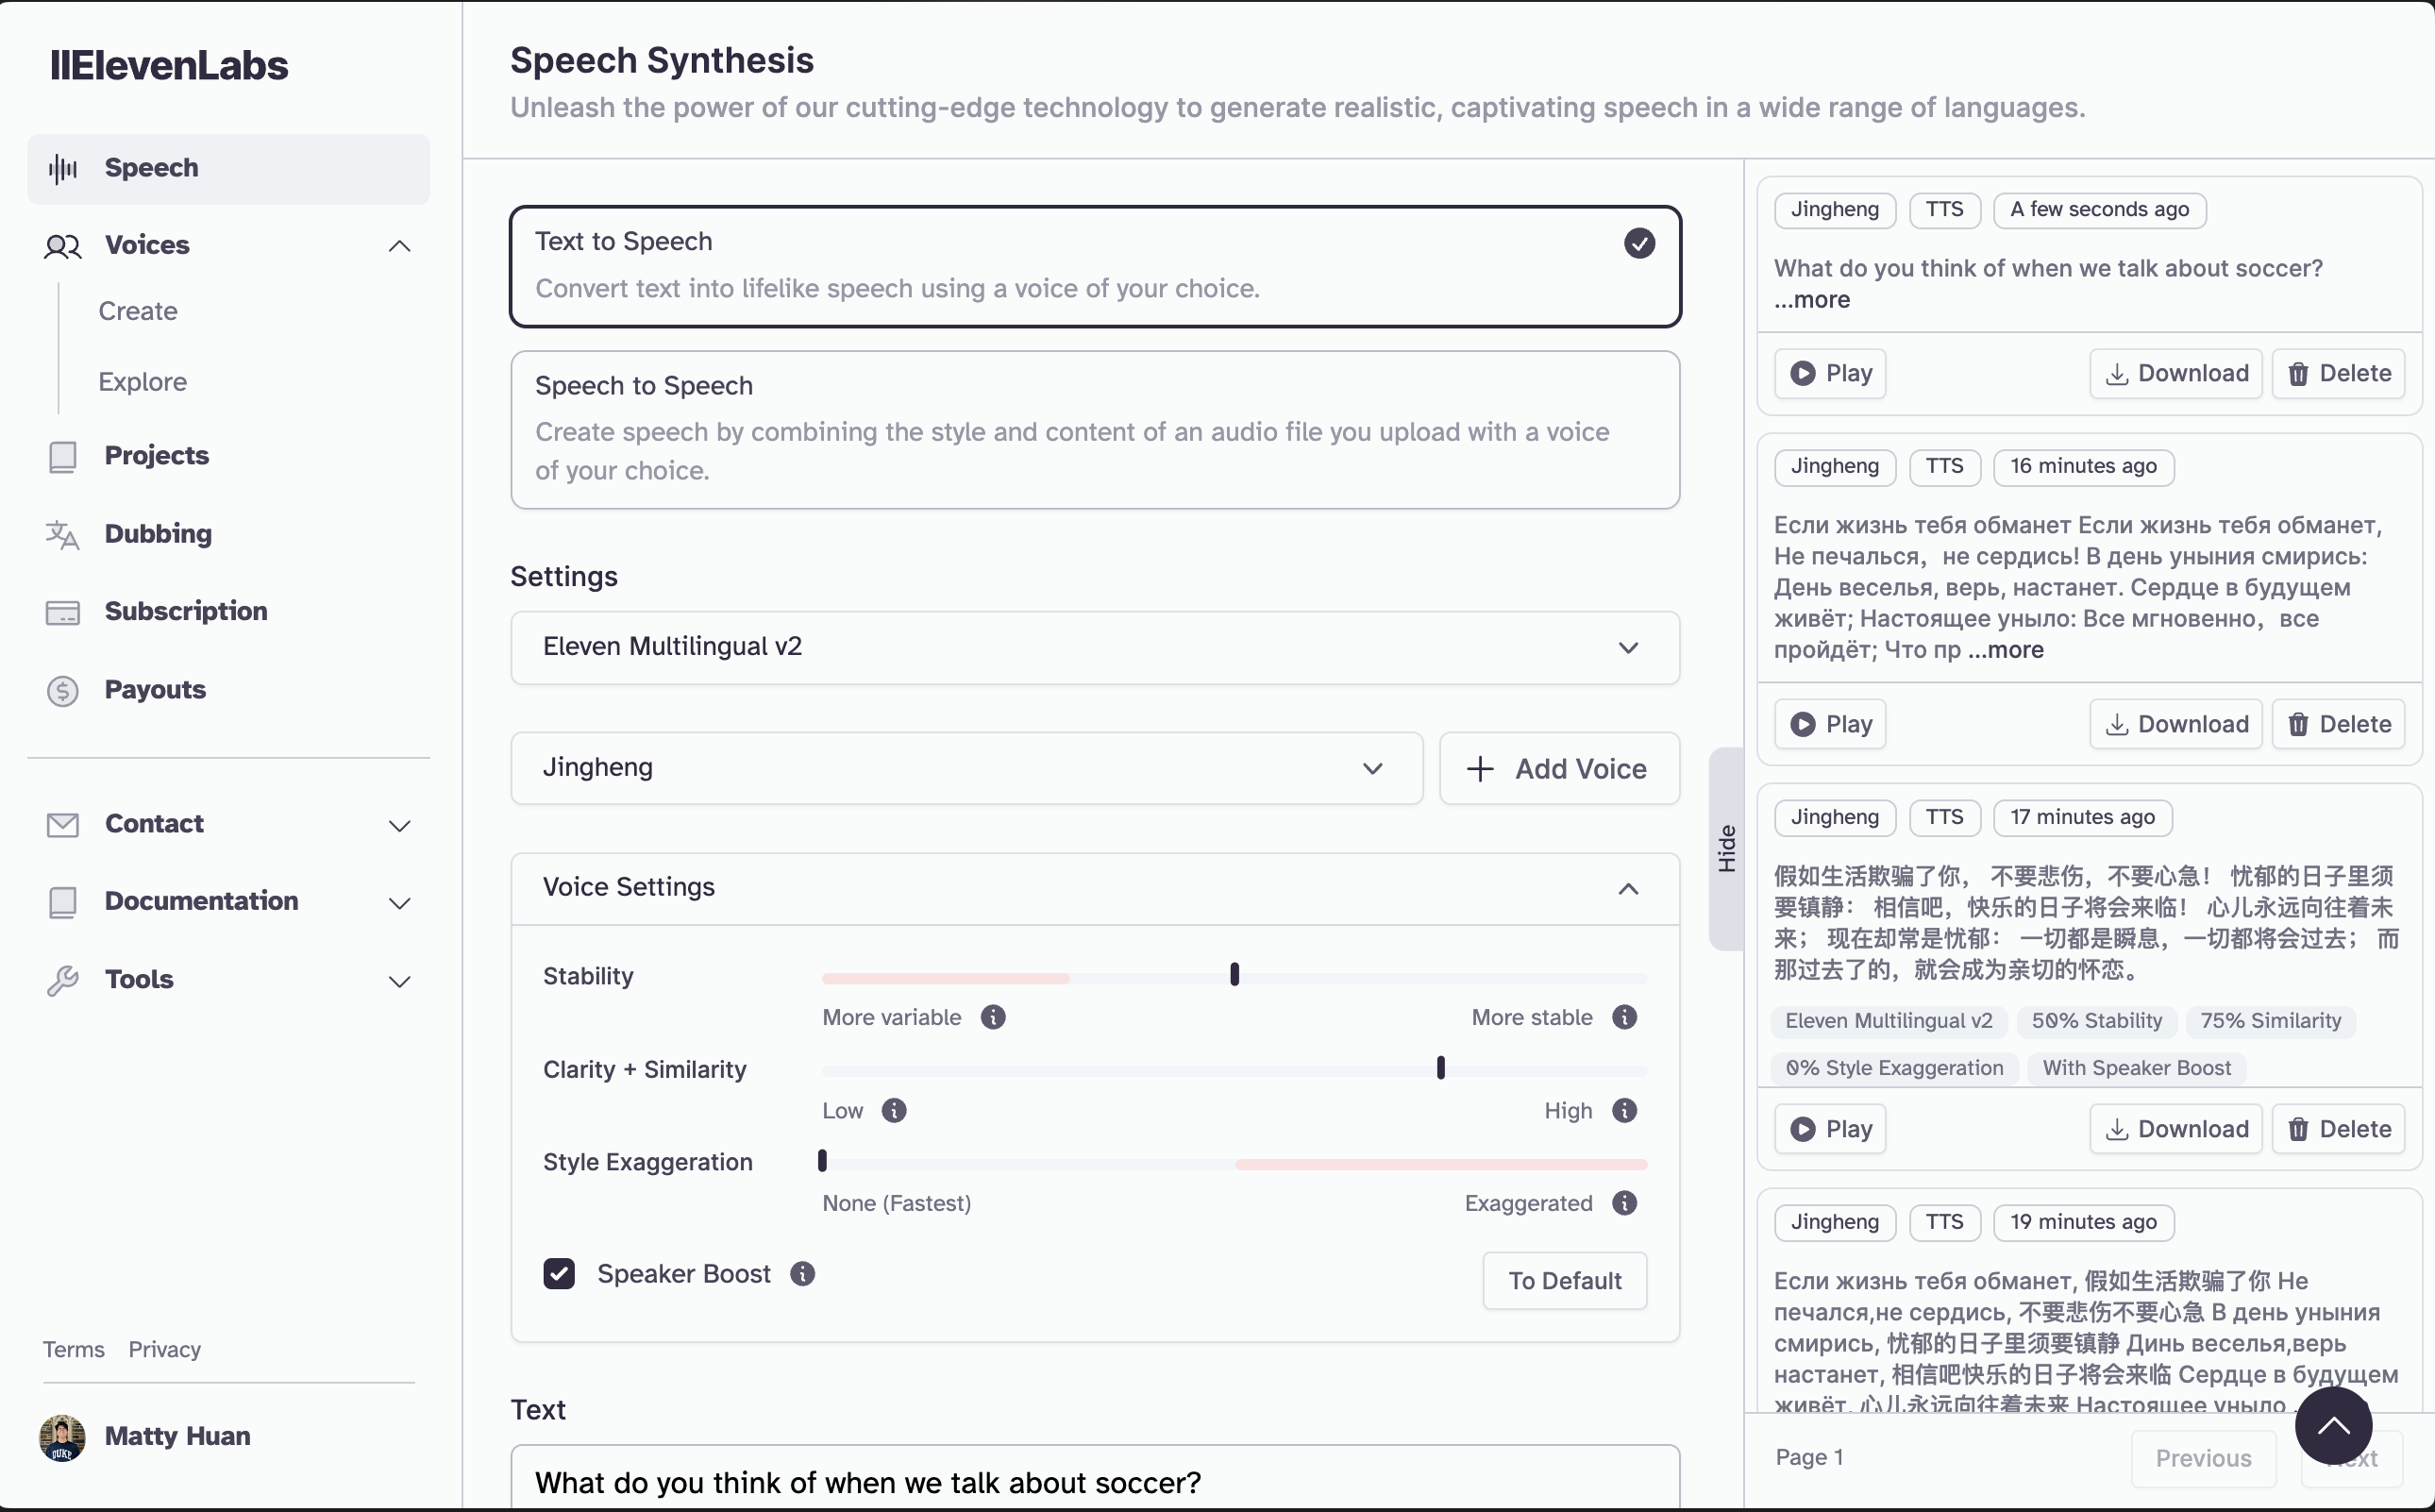
\includegraphics[width=0.8\textwidth]{ElevenLabs.png}
  \caption{Using my clone voice to generate the voice over for the video, I recorded the training set by reading one chapter from the book \textit{Elon Musk}, the audio file is 14 mins.}
\end{figure}

ElevenLabs, positioned at the forefront of AI-driven audio synthesis, particularly in voice cloning and text-to-speech (TTS) technologies, likely utilizes Recurrent Neural Networks (RNNs), Long Short-Term Memory (LSTM) units, and Autoregressive Transformers. 
These models excel in understanding and generating the temporal sequences crucial in replicating human speech's nuanced dynamics. 
While ElevenLabs has not publicly disclosed the specific models underpinning its technology, the theoretical basis of these models provides a clue to the sophisticated mechanism that enables ElevenLabs to produce highly realistic and expressive voice outputs. 
RNNs and LSTMs could be instrumental in modeling the sequential nature of speech, capturing the temporal dependencies necessary for coherent speech generation. 
Autoregressive Transformers, with their powerful self-attention mechanisms, offer a means to process long sequences in parallel, potentially enhancing the system's ability to manage the structure of speech at scale. 
Together, these models could form the basis of ElevenLabs’ ability to analyze and replicate the unique attributes of individual voices, offering voice synthesis capabilities that find applications in entertainment, education, and beyond.

%%%%%%%%%%%%%%%%%%%%%%%%%%%%%%%%%%%%%%%%%%%%%%%%%%%%%%%%%%%%%%%%%%%%%%%%%%%%%%%%

\chapter{Performance Evaluation}

\section{Overview of Project Outcome}

This video project is a mix of the latest AIGC tools and creative ideas, presents a narrative that is both visually stunning and thematically profound. 
It tells a story in one minute with series of crafted scenes, each contributing to a cohesive storyline that explores the symbiotic relationship between humanity and AI-driven robots.
It is set in a futuristic landscape, the narrative delves into themes of the potential futures shaped by the integration of advanced AI entities within human society. 
This thematic exploration is brought to life through a variety of scenes, ranging from peaceful, digitally-rendered natural view to bustling, urban technology alive with the vibrancy of cyber-punk life. 
The selection and progression of scenes are carefully arranged to not only captivate the audience with visual magnificence but also to provoke thought and reflection on the evolving role of AI in our world.

The project's success in delivering a narrative is largely attributable to the use of AI technologies at each stage of the creative process. 
From the generation of high-fidelity image stills with Midjourney to the video synthesis facilitated by Runway Gen-2, the tools represent the potential of AI to the traditional boundaries of content creation. 
The narrative is further enriched with a voiceover, rendered through ElevenLabs' voice cloning technology, adding a layer of narrative depth that guides the audience through the unfolding story. 
This integration of AI-driven voice synthesis not only enhances the immersive quality of the video but also demonstrates the potential of AI in crafting engaging and emotionally resonant storytelling. 
The video's aesthetic and thematic achievements are underscored by Topaz AI, which elevates the visual quality through enhancements such as frame rate optimization and noise reduction, ensuring that the final product has a good overall quality.

This project, through its combination of AI capabilities and creative narrative design, opens a dialogue on the future of storytelling in the age of artificial intelligence. 
It stands as an example of how AI support to create content that is not just visually captivating, but also rich in thematic depth, challenging us to envision the limitless possibilities of creative expression in the digital era.

\section{Deliverable Analysis}

\begin{figure}[htbp]
  \centering
  \includegraphics[width=0.9\textwidth]{AudioPreview.png}
  \caption{Spectral and waveform analysis of an MP3 file displayed in a sound engineering interface.}
\end{figure}

The image presents a visualization of an MP3 file's acoustic properties with details about a spectrum analyzer interface. 
The vibrant colors map out varying degrees of sound intensity across a broad frequency range, while the graphical representations below reveal the waveforms and their amplitudes. 
This visualization shows audio quality but also serves as a critical tool for engineers seeking to understand and manipulate the nuanced differences.

\newpage

\begin{figure}[htbp]
  \centering
  \includegraphics[width=0.8\textwidth]{Start.png}
  \caption{Silhouettes watching a glowing soccer ball, evoking pre-match anticipation.}
\end{figure}

A group of silhouetted crowds can be seen in this photograph looking toward a bright soccer ball.
It seems as though there is a moment of silent expectancy. 
The ball appears to be floating in a spotlight, acting as a focal point and scene-setter for an excitement.
This silence creates an atmosphere of anxiety leading up to the game, as if everyone is holding their breath until it starts. 
It shows the charm of soccer game, which brings together supporters worldwide.

\newpage

\begin{figure}[htbp]
  \centering
  \includegraphics[width=0.8\textwidth]{Stadium.png}
  \caption{The World Cup stadium, a modern architectural wonder with crazy fans.}
\end{figure}

The image captures the vibrant energy of a stadium filled with soccer fans. 
The architecture is a modern engineering, with elegant curves and beams that arch towards the sky, illuminated by lights that cast a warm glow over the attendees. 
The field is a bright patchwork of greens, set against the darker hues of the spectator stands.
This is more than a stadium; it's a center of excitement, where every cheer and gasp is amplified, and every moment is considered as collective memory of the global soccer community.

\newpage

\begin{figure}[htbp]
  \centering
  \includegraphics[width=0.8\textwidth]{Cheering.png}
  \caption{Excited fans painted in team colors cheer passionately at a soccer match.}
\end{figure}

The photograph showcases a jubilant fan, her face is like a canvas of vibrant national colors.
Their excitement collectively embodies the passionate heart of the soccer world. 
This display of emotion and unity displays the profound connection between the fans and the beautiful game.

\newpage

\begin{figure}[htbp]
  \centering
  \includegraphics[width=0.8\textwidth]{Star.png}
  \caption{A soccer player in a celebration, symbolizing the sports success.}
\end{figure}

The image vividly captures the moment of victory. 
As he looks towards the sky, the raw emotion of success washes over his features.
Confetti rains down like colorful blessings, blending with the beads of sweat and tears of joy that mark this achievement. 
It is a snapshot that touches upon the deeply human experience of reaching a long-sought goal.

\newpage

\begin{figure}[htbp]
  \centering
  \includegraphics[width=0.8\textwidth]{Steal.png}
  \caption{A skilled midfielder skillfully navigating the opposition in a heated match.}
\end{figure}

The dynamic image showcases a midfielder in action.
The player's hair is caught mid-flight, a wild mane that echoes their untamed skill.
It is a ballet of athleticism, where precision meets passion, and the raw fervor of the game comes to life with every touch and turn.
\newpage

\begin{figure}[htbp]
  \centering
  \includegraphics[width=0.8\textwidth]{Victory.png}
  \caption{A team celebrates a goal, uniting in victory under the stadium lights.}
\end{figure}

The photograph captures the zenith of a soccer match.
It is a joy that spreads through the air like a wave, enveloping teammates in a tight circle of collective triumph. 
It is a scene that concludes the shared passion and glory that is the spirit of the sport.
\newpage

\begin{figure}[htbp]
  \centering
  \includegraphics[width=0.8\textwidth]{NewStadium.png}
  \caption{A modern stadium glows under advanced lighting, ready for a historic soccer final.}
\end{figure}

Under the lights, the stadium emerges as a triumph of modern architecture. 
Its design is a fusion of nature's curves and the sharp angles of contemporary technologies.
Hovering displays pulse with data, providing a stream of information as tangible as the excitement that fills the air. 
Here, every seat hums with the energy of thousands, all awaiting this miracle of soccer achievement.
\newpage

\begin{figure}[htbp]
  \centering
  \includegraphics[width=0.8\textwidth]{Open.png}
  \caption{Robots in team colors perform a precise pre-game warm-up inside the stadium.}
\end{figure}

As the stadium buzzes with anticipation, a line of robots glides across the polished floor with the grace of seasoned athletes, these machines perform their pre-game routine. 
Each robot, with team colors that gleam in the arena's lights, moves with a precision that belies the passionate chaos of the game to come. 
This dance of steel and light is as much a part of the spectacle as the match itself, promising a competition where human creativity and robotic excellence meet.
\newpage

\begin{figure}[htbp]
  \centering
  \includegraphics[width=0.8\textwidth]{Ball.png}
  \caption{Smart soccer ball with glowing design, ready for kickoff at center circle.}
\end{figure}
At the heart of the field lies a futuristic soccer ball, a centerpiece of innovation, poised at the center circle. 
Its surface is a array of glowing patterns, signaling its smart capabilities that capture and interact with every play. 
A player steps forward, foot grazing the ball in a light tap that sparks a radiant glow, signaling the start of something more than just a game; 
it's a dance of agility and intelligence, where every movement is tracked and analyzed, ready to begin with the referee's whistle.
\newpage

\begin{figure}[htbp]
  \centering
  \includegraphics[width=0.8\textwidth]{Kick.png}
  \caption{Robotic player and smart ball at the high-tech kickoff.}
\end{figure}

The commencement of the game is an exhibition of technological capabilities, as a robotic figure executes the initial kick with calculated precision. 
The soccer ball reacts to the contact with a surge of internal light, its advanced circuitry capturing and broadcasting the game's dynamics. 
The spectacle of lights and data animation not only signals the start of the match but also shows the fusion of sport and cutting-edge technology.
\newpage

\begin{figure}[htbp]
  \centering
  \includegraphics[width=0.8\textwidth]{Green.png}
  \caption{Players warm up on an interactive, light-responsive field.}
\end{figure}

As the stadium hums with anticipation, players take to the field, their silhouettes casting long shadows in the green glow of the technologically enriched turf. 
They engage in a ballet of stretches and strategic drills, each movement traced by the intelligent lighting system beneath their feet, a dance of light and shadow playing out across this amazing stage.
\newpage

\begin{figure}[htbp]
  \centering
  \includegraphics[width=0.8\textwidth]{RobotCelebration.png}
  \caption{A robot scores with precision, celebrated by a light show.}
\end{figure}

In this electrifying scene, the fusion of advanced robotics and the game of soccer reaches its climax. 
A robotic striker, with perfect precision, sends the ball soaring from the penalty box into the mesh of the net. 
As the goal is scored, the stadium's net bursts into an animated light show, with digital fireworks in celebration. 
\newpage

%%%%%%%%%%%%%%%%%%%%%%%%%%%%%%%%%%%%%%%%%%%%%%%%%%%%%%%%%%%%%%%%%%%%%%%%%%%%%%%%


\section{Limitation of Current AIGC tools}

GPT-4, despite its evolution over previous iterations, carries inherent limitations that affect its utility for continuous, intensive use. 
For paid users, a notable restriction is the allowance of only 40 messages every 3 hours. 
This cap hinders users from using the AI for heavy-duty tasks, impacting productivity for those relying on it for extensive content creation.
Furthermore, GPT-4's large language model, while impressive, can sometimes be a double-edged sword. 
The AI's propensity to use advanced vocabulary and complex sentence structures can make its outputs less accessible, particularly for non-native English speakers or individuals with varying levels of language proficiency. 
This linguistic barrier can render image descriptions and other generated content obscure, reducing the effectiveness of communication and limiting the user experience.

Midjourney, even though considered as state-of-the-art image generation model, also encounters its set of challenges. 
One significant drawback is its operation exclusively through Discord, complicating the onboarding process and detracting from user convenience. 
This barrier not only adds unnecessary steps for users to get familiar with using Discord, but also raises privacy concerns on a public server where activities are visible to all. 
Additionally, Midjourney's strict content censorship, aimed at maintaining PG-13 content, can inhibit creativity. 
This rigorous moderation limits users' freedom to explore diverse themes, impacting the breadth of creative expression possible with the tool. 
The AI model's struggle with context understanding further compounds these limitations. 
It often fails to grasp the details of prompts, especially in specialized domains, leading to outputs that may not align with users' intentions.

Runway's Gen-2 model, while pioneering in the text-to-video domain, exhibits limitations that underscore the challenges in current AI video generation technology. 
Its inability to fully comprehend user prompts, particularly those involving motions, results in videos where characters and objects may unnaturally merge or separate. 
This necessitates additional input from users, like employing the motion brush tool to dictate character movements, making it more time-consuming for the creation process. 
Furthermore, the generated videos occasionally suffer from a low frame rate and a noticeable graininess, diminishing the overall quality of the output. 
Such drawbacks make post-production editing necessary to achieve a polished product, detracting from the efficiency and appeal of using AI for video generation. 
Moreover, the model's struggle with capturing motion accurately can lead to unsettling video outputs, undermining the potential for its application in professional or creative projects.

Topaz AI focuses on image and video processing, particularly through techniques such as upscaling, noise removal, and subject sharpening. 
The tool's ability to significantly improve the resolution and quality of digital media showcases the potential of AI in enhancing visual content. 
However, the substantial computing power required by Topaz AI introduces a notable limitation, as users often find their systems bogged down during processing, rendering them incapable of multitasking. 
This highlights a critical area for improvement: optimizing AI tools to minimize their demand on computing resources while maintaining their output quality. 
Despite these challenges, the development brought by Topaz AI in delivering high-quality visual content quickly and efficiently cannot be understated. 
As the tool continues to evolve, future iterations will likely address these computational efficiency issues, making it an even more indispensable asset for creators seeking to elevate their visual content to new heights.

ElevenLabs' strides in voice synthesis technology, particularly through its "Professional Voice Cloning" feature, have showcased the remarkable capability of AI to mimic human voices with impressive accuracy. 
However, this process requires a significant investment of time — three hours for audio recording plus a six-hour wait for processing — points to a bottleneck in efficiency, potentially slowing down creative workflows and project timelines. 
Despite these obstacles, the customized outcome of the cloned voices, which closely resemble their human counterparts, underscores AI in capturing the essence of human speech. 
Yet, the difference between synthesized and real voices remains a problem to conquer, indicating that while ElevenLabs has made considerable progress, there is still a journey ahead towards indistinguishable voice cloning that combines integration with faster processing times.

\section{Ethical Considerations}

The development of generative text-to-image models has brought forth the ethical considerations that these models may cause. 
Notably, biases towards certain genders or skin tones have been observed in the outcomes of these image generation models. 
To offset this, a novel approach has been proposed \cite{esposito2023mitigating}, which involves fine-tuning text-to-image models on synthetic data constructed from diverse text prompts. 
These prompts include a variety of perceived skin tones, genders \cite{buolamwini2018gender}, ethnicities, professions, and age groups, resulting in a more inclusive synthetic dataset. 
Fine-tuning models with this diverse data has shown to substantially improve group fairness metrics, reducing biases by significant margins.
The process begins with the construction of text prompts through multiplicative combinations of various social qualifiers, which are then used to synthesize images that showcase a broad spectrum of human diversity. 
This method has proven to be effective, with diversity-finetuned models not only generating content that is more representative of darker skin tones and female genders but also improving overall fairness in model outcomes.

Furthermore, the evaluation of biases in text-to-image models is formulated within a fairness framework \cite{selbst2019fairness}, which assesses whether model outputs unfairly favor certain subgroups over others. 
By adopting this framework, the research moves beyond merely measuring bias to actively promoting fairness in AI-generated content. 
This is complemented by user studies that validate the absence of undesirable visual artifacts in finetuned models' outputs.
This approach not only showcases the capability to generate more inclusive content but also highlights the potential for AI to serve as a tool for social change. 
By actively mitigating biases, AI models can foster digital environments that are reflective of a wide spectrum of human experiences and perspectives, thereby promoting inclusivity and diversity.
Future work need to address additional forms of biases and explore the applicability of mitigative strategies in video models, thereby extending the principles of fairness and inclusivity to broader multimedia contexts.

The ethical deployment of AIGC also necessitates the establishment of robust regulatory frameworks and self-regulatory practices within organizations. 
Familiarizing oneself with national and international regulations pertaining to data privacy, consumer protection, and intellectual property rights is essential for compliance. 
Furthermore, the adoption of self-regulatory measures, such as transparent disclosure of AI involvement in content creation \cite{diakopoulos2016accountability} and the implementation of quality control measures, is vital for maintaining the trust and confidence of users.
Transparency in the use of AIGC is a cornerstone of ethical practice. 
Businesses must clearly communicate the role of AI in generating content, enabling users to make informed decisions. 
Moreover, quality control mechanisms must be instituted to ensure the accuracy, relevance, and appropriateness of AI-generated content. 
Protecting user privacy and securing personal data against unauthorized access is another critical aspect that businesses must rigorously uphold.
By ensuring regulatory compliance, and adhering to best practices for transparency and quality control, we can enrich the digital landscape while respecting the ethical consideations of equity, privacy, and accountability.

%%%%%%%%%%%%%%%%%%%%%%%%%%%%%%%%%%%%%%%%%%%%%%%%%%%%%%%%%%%%%%%%%%%%%%%%%%%%%%%%

\chapter{Conclusions}
\label{conclusions}

In conclusion, the exploration of AIGC technologies in this SW report has illuminated the potential of AI in reshaping digital content creation. 
Through the utilization of advanced models such as GPT-4, Midjourney, Runway, ElevenLabs and Topaz AI, we have demonstrated the capability of AI to not only augment but also reform the processes of generating text, images, videos, and synthesized voice. 
The case study focused on envisioning the future of soccer provided a practical application of these technologies, displaying how they can create immersive and narrative-rich content. 
Despite the remarkable developments, the journey uncovered inherent limitations within current AIGC tools, highlighting areas for further evolution to enhance accessibility, user experience, and the quality of AI-generated content.

Ethical considerations also emerged as a critical aspect of deploying AIGC technologies. 
The report delved into the challenges posed by biases in text-to-image models and the importance of implementing strategies to ensure fairness and diversity in AI-generated content. 
It emphasized the need for transparency, adherence to regulatory frameworks, and the implementation of quality control measures as essential practices for responsible AI use. 
These ethical guidelines navigate the AIGC, ensuring that the development and application of these technologies contribute positively to society and respect individual rights and dignity.

As we stand on the edge of a new era in digital content creation, fueled by AI innovations, this SW underscores the balance between embracing the possibilities offered by AIGC and addressing the ethical and technical challenges it presents. 
The future of AIGC holds immense promise for creative expression and storytelling, inviting us to reimagine the boundaries of what is possible. However, it also calls for a concerted effort among developers, users, and policymakers to foster a responsible environment. 
As we move forward, the lessons learned from this exploration will undoubtedly shape the trajectory of AIGC, guiding us towards a future where AI empowers humanity to create, inspire, and connect in ways we are only beginning to imagine.

%%%%%%%%%%%%%%%%%%%%%%%%%%%%%%%%%%%%%%%%%%%%%%%%%%%%%%%%%%%%%%%%%%%%%%%%%%%%%%%%

\chapter*{References}
\label{references}
\addcontentsline{toc}{chapter}{References}



\printbibliography[heading=none]


%%%%%%%%%%%%%%%%%%%%%%%%%%%%%%%%%%%%%%%%%%%%%%%%%%%%%%%%%%%%%%%%%%%%%%%%%%%%%%%%

\appendix

\chapter{Additional Material}
\label{appendix-a}

The link of the video is here: \url{https://youtube.com/shorts/C_Ng1JBiA-c?feature=shared}

\end{document}